\documentclass[12pt]{article}
\usepackage{times}
\usepackage{babel}
\usepackage{titling}
\usepackage{amsmath,amssymb,amsfonts}
\usepackage{graphicx}
\usepackage{setspace}
\usepackage{cite}
\usepackage{textcomp}
\usepackage{xcolor}
\usepackage{multirow}
\usepackage{booktabs}
\usepackage{subcaption}
\usepackage{hyperref}

\usepackage[%
    left=2cm,%
    right=2cm,%
    top=3cm,%
    bottom=3cm,%
    paperheight=29.7cm,%
    paperwidth=21cm%
]{geometry} % Page settings

\onehalfspacing

\begin{document}
\begin{titlepage}

\setlength{\droptitle}{-4em}
\center

{\huge \bfseries Recursive Belief Vision Language Action Models} % Title of the project
\\[2cm]

\begin{minipage}{0.6\textwidth}
\begin{center} \large
Submitted by: \textbf{Vaidehi Bagaria} \\[0.5cm]
Registration no: \textbf{ED21B070}
\end{center}
\end{minipage}

\vspace{8em}


\includegraphics[width=4cm]{logo.pdf}

\vspace{8em}
\begin{minipage}{0.6\textwidth}
\begin{center} \large
\textbf{Engineering Design and IDDD Robotics} \\[0.5cm]
\textbf{Dual Degree Project Report}
\end{center}
\end{minipage}

\vspace{4em}
{\large \today}

\end{titlepage}

\begin{abstract}
\noindent Vision-language-action models must enable agents to execute long-horizon tasks under partial observability. However, most existing approaches remain observation-driven, relying on short context windows or repeated queries to vision-language models (VLMs). This leads to loss of task progress, action repetition under perceptual aliasing, and high inference latency. While semantic grounding is important, long-horizon manipulation fundamentally requires persistent, action-conditioned state representations. Current VLAs lack such representations and exhibit limited temporal and physical reasoning, making them ill-suited for multi-stage control.

This report introduces Recursive Belief (RB)-VLA, a belief-centric architecture trained with self-supervised world-model objectives that maintains a compact latent state for encoding task-relevant history, dynamics, and object interactions. Queried once per task, the VLM provides high-level intent, while the belief tracks task progress and enables phase-aware, causally grounded control under partial observability without storing raw observations or scaling memory with time. The belief and intent jointly condition a diffusion policy for robust closed-loop execution.

RB-VLA outperforms prior VLAs on long-horizon benchmarks, achieving 52.5\% and 32.5\% higher success rates on multi-stage pick-and-place and stacking tasks, respectively, compared to $\pi_0$. It also reduces inference latency by up to $5\times$ relative to baselines and eliminates memory growth across timesteps observed in existing VLAs. The model demonstrates increased robustness under occlusion and more consistent task progression in multi-stage settings. Ablations show the belief module is the primary driver of performance, increasing success rates from 32.5\% without belief to 77.5\% with belief. These results demonstrate the effectiveness of belief-based state representations for long-horizon, multi-stage control.
\end{abstract}

\section{Introduction}

\subsection{Background and Motivation}
Robotic manipulation has long been a central problem in artificial intelligence and robotics, requiring an agent to perceive its environment, reason about object relationships, and produce continuous, physically grounded actions. Recent progress in foundation models has enabled vision--language--action (VLA) systems that combine large-scale visual and linguistic representations with action prediction, allowing robots to follow natural-language instructions and generalize across tasks. By replacing brittle hand-engineered pipelines with a unified, instruction-conditioned interface, VLAs offer a scalable path toward general-purpose manipulation.

Despite this progress, deploying VLAs to real-world settings remains difficult, particularly for long-horizon, multi-stage manipulation tasks where the meaning of an action depends on what has happened before. In such settings, observations are inherently partial: objects become occluded by the gripper or the environment, lighting and viewpoint vary, and visually similar objects induce perceptual aliasing. A policy that conditions only on the current observation cannot disambiguate task state, leading to action repetition, regression, or outright failure. Effective control therefore requires a persistent, action-conditioned representation of task progress, not merely accurate semantic perception of the current frame. This work investigates how such a representation can be learned and maintained efficiently within a VLA, without sacrificing the semantic generalization that makes VLAs attractive in the first place.

\subsection{Limitations of Current Approaches}
Vision--language--action models \cite{kim2024openvla,ye2025vla,zitkovich2023rt} have shown strong generalization by combining language understanding with visual perception to directly produce robot actions, improving scalability over classical control systems. However, most VLAs implicitly adopt a Markovian assumption, conditioning actions only on the current observation or a short history window \cite{jang2025contextvla,lin2025hif,wang2025lola}. Such reactive reasoning fails to capture long-term context under noisy observations, perceptual aliasing, occlusion and temporally static short observation histories. This limitation reduces its effectiveness for long-horizon, multi-stage, partially observable real-world manipulation. While longer context could address this, current VLAs scale memory through token accumulation, resulting in high latency and unreliable task state retention. Effective decision-making therefore requires reasoning over past actions and their consequences through compact state representations.

Some approaches rely on defining multi-stage dynamics with explicit task-stage supervision for long-horizon behavior \cite{xu2025stare,ji2025robobrain}. However, manipulation is driven by smoothly evolving, action-grounded internal dynamics rather than discrete labels. Learning continuous dynamics better captures shared physical structure across tasks, whereas stage-based supervision is task-specific and poorly generalizable.

World models \cite{chen2022transdreamer} address this by modeling agent--environment dynamics, enabling future-aware planning in VLAs. Although vision--language models excel at semantic inference, they lack explicit grounding in physical dynamics and state evolution, ignoring physical constraints \cite{gao2025vision}. World models bridge this gap by linking visual observations to action-conditioned dynamics that enable reasoning about future states beyond semantics alone. Existing approaches refine VLM decisions by predicting future observations with world models for online correction \cite{feng2025reflective,wang2025vagen,cen2025worldvla}, but rely on repeated, computationally expensive dynamic rollouts. In contrast, maintaining a compact internal belief state that tracks task progress through the consequences of past actions, enables action selection without continual forward simulation at each timestep.

\begin{figure}[!htbp]
\centering
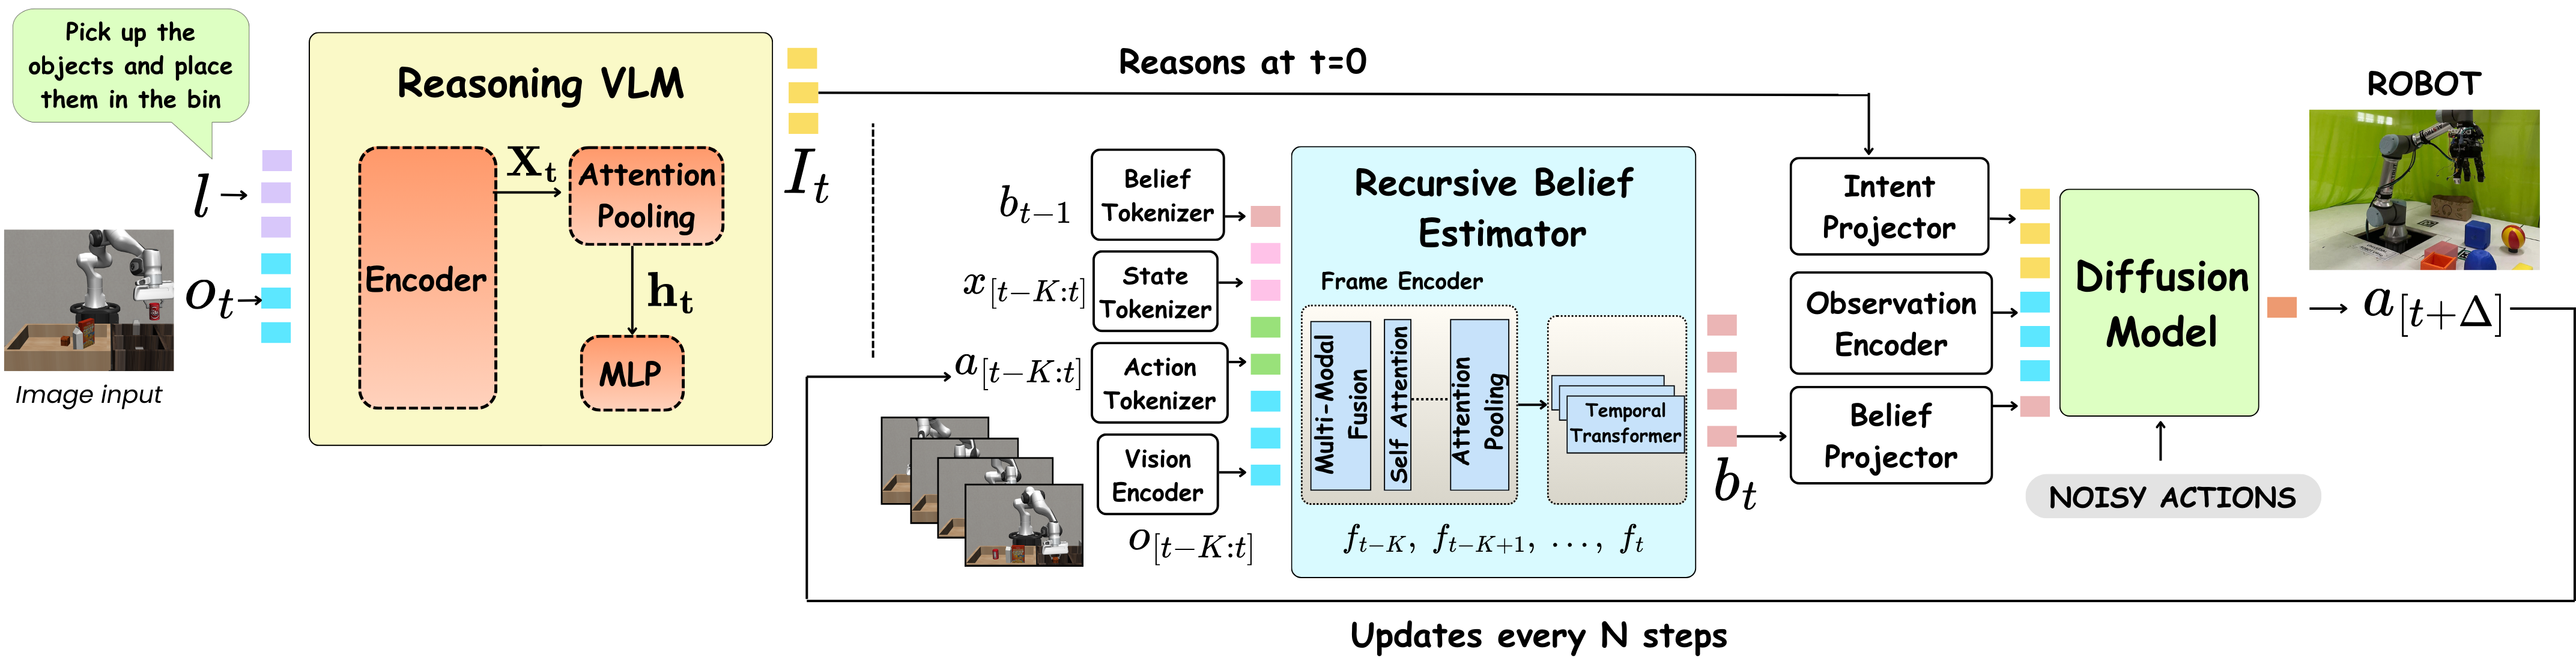
\includegraphics[width=\textwidth, keepaspectratio]{main_new.png}
\caption{\textbf{Overall Architecture of RB-VLA}. (a) A VLM generates high-level intent from the current observation and instruction at $t=0$, implicitly grounding task semantics and relevant scene entities. (b) Recursive belief estimator maintains a compact belief encoding task-relevant history. (c) A DiT-based action head generates action chunks for closed-loop control.}
\label{fig:block}
\end{figure}

In the absence of an internal state, VLAs repeatedly re-interpret observations with VLMs, leading to high computational cost and latency. Since VLMs provide semantic abstraction, they can be invoked sparsely, while causal reasoning governs low-level task execution. Hierarchical approaches improve computational efficiency and robustness by decoupling planning and control for long-horizon tasks \cite{li2025towards,zhang2025hierarchical}. However, they still struggle with memory and task awareness.

\subsection{Contributions}
To address these issues, we introduce the Recursive Belief VLA (RB-VLA) framework. Our key contributions are:
\begin{enumerate}
\item \textbf{Belief-centric VLA formulation:} We introduce a fixed-size, action-conditioned recursive belief memory that captures task-relevant interaction history and system dynamics, enabling causal reasoning and consistent decision-making under partial observability.
\item \textbf{Phase-aware long-horizon control:} The recursive belief provides short and long-horizon predictive context, supporting implicit phase estimation and conditioning a diffusion policy for dynamics-consistent closed-loop control in place of short observation windows.
\item \textbf{Decoupled semantic grounding and control:} We treat semantic reasoning as episodic by querying a VLM once to extract grounded task intent, eliminating dense semantic re-inference.
\item \textbf{Empirical validation on long-horizon benchmarks:} We demonstrate substantial improvements on long-horizon, multi-stage manipulation tasks and under occlusion, outperforming prior VLAs while maintaining constant memory usage and significantly lower latency.
\end{enumerate}

\section{Literature Review}

\subsection{Vision--Language--Action Models}
Recent vision--language--action models \cite{kim2024openvla,brohan2022rt} remain reactive by framing control as autoregressive action token prediction using large language models. While effective for semantic alignment, invoking a full language model at every step to produce only a small number of action tokens is computationally expensive. Prior work attempts to reduce this cost through chunked or parallel decoding \cite{kim2025fine,song2025accelerating}, selective activation \cite{yang2025efficientvla}, and visual token compression \cite{vasu2025fastvlm}. However, discrete action token prediction limits smooth continuous control and precise multimodal action generation, motivating recent approaches that replace the language head with continuous action decoders, such as diffusion \cite{bjorck2025gr00t} or flow-based policies \cite{black2025pi_}. These approaches nevertheless remain fundamentally observation-driven, relying on dense semantic re-inference that recomputes the same goals and instructions at every step. RB-VLA addresses these limitations by maintaining a persistent state that tracks task progress and replaces computationally heavy VLM-based reinterpretation.

\subsection{Long Horizon Manipulation}
Long-horizon, multi-stage manipulation requires policies to reason over extended interactions. Existing approaches introduce inductive structure for long horizon tasks by explicitly predicting subgoals \cite{yang2025lohovla} or by conditioning policies on manually defined motion phases \cite{fan2025long}. While effective for skill chaining and temporal abstraction, these methods rely on task-specific subtask or phase supervision.

Some recent methods improve reasoning by introducing explicit intermediate inference before action selection. ECoT \cite{zawalski2024robotic}, ThinkAct \cite{huang2507thinkact}, and related approaches \cite{zhao2025cot,li2025coa} generate visually grounded reasoning over sub-tasks, affordances, or latent plans to condition action prediction. Although these methods improve reasoning and reduce hallucination, they operate primarily in image--text space and lack persistent awareness of task progress, often failing in multi-stage execution. This motivates belief-based dynamics-grounded representations that summarize interaction history and enable robust closed-loop long-horizon behavior.

\subsection{Memory and Context}
As interaction history grows unbounded over time, relying on noisy raw or compressed observation windows over long horizons becomes infeasible. Short histories discard task-critical temporal information, leading to failure under perceptual aliasing and in visually static multi-stage scenarios \cite{spaan2012partially}. In RB-VLA the belief instead provides a fixed-size, dynamics-consistent memory that filters observation noise and selectively retains motion-relevant information from past interactions and dynamics.

Some prior works incorporate history through recurrent features \cite{xiao2025ava} or growing memory tokens over time \cite{koo2025hamlet}, but these mechanisms do not explicitly ground memory in action-conditioned dynamics. Other approaches learn long-horizon memory via selective context retention and gated fusion \cite{liu2025evovla}, where memory primarily serves as a post-hoc modulator of policy outputs rather than an internal state that shapes perception and encodes action-induced transitions. Predictive world-model methods explicitly model dynamics and generate dense future rollouts for planning or inference \cite{cen2025rynnvla, liu2025trivla}, while classical belief-space planners rely on explicit models and forward simulation \cite{kaelbling2013integrated}. Both incur substantial computational overhead and limit real-world applicability.

Using world-model training objectives, RB-VLA learns a belief state sufficient for future prediction, without heavy rollout-based forward simulation at inference. The belief recursively modulates perception toward interaction-driven dynamics.

\section{Objectives}
The objectives of the proposed project are:
\begin{enumerate}
    \item To formulate a belief-centric vision--language--action architecture that maintains a fixed-size, action-conditioned recursive memory capturing task-relevant interaction history and system dynamics, enabling causal reasoning and consistent decision-making under partial observability.
    \item To enable phase-aware long-horizon control by using the recursive belief as both short- and long-horizon predictive context, supporting implicit phase estimation and conditioning a diffusion policy for dynamics-consistent closed-loop control in place of short observation windows.
    \item To decouple semantic grounding from control by treating vision--language reasoning as an episodic, one-shot operation that produces a grounded task intent, thereby eliminating dense per-step semantic re-inference and reducing inference latency.
    \item To empirically validate the proposed framework on long-horizon, multi-stage manipulation tasks in simulation and on real hardware, demonstrating improved success rates under partial observability, constant memory usage, and significantly lower latency relative to prior VLAs.
\end{enumerate}

\section{Methodology}

\subsection{System Overview}
Long-horizon manipulation is formulated as a partially observable control problem with a learned belief estimator. The belief links perception to underlying motion dynamics rather than relying on raw observations, providing invariance to visual and environmental variation.

The system consists of three components (Fig.~\ref{fig:block}): a vision--language reasoning module, a belief estimator, and a diffusion-based controller. We decouple semantic task specification from causal state estimation: a vision--language model is queried sparsely to extract a static latent goal embedding $I_t$ from language and initial observations, binding instructions to concrete objects in the scene. This grounded goal embedding remains fixed throughout execution, as object identity and task semantics are static.

At each step, the belief estimator integrates the previous belief $b_{t-1}$, a window of tokenized observations $o_{t-K:t}$, actions $a_{t-K:t}$, and proprioceptive states $x_{t-K:t}$ (end-effector pose, velocity, acceleration and force--torque measurements) using a temporal transformer to produce a latent belief $b_t$ that tracks physical interaction progress. Low-level control is executed by a diffusion policy conditioned on $(b_t, I_t)$, operating in closed loop at high frequency.

Conceptually, the belief acts as a learned, recursively-updated sufficient statistic of task-relevant history. Whereas raw observation windows must trade off horizon length against memory and latency, the belief compresses arbitrarily long interaction history into a fixed-dimensional vector whose contents are shaped by the world-model training objective rather than by hand-designed memory rules.

\subsection{Belief Estimator}
\label{subsec:belief}
Long-horizon execution under partial observability is enabled by maintaining a belief state that captures information unavailable at a single timestep, such as occluded object states, contact history, and interaction progress, while being recursively updated and fixed in dimensionality. Similar to a state estimator \cite{chen2003bayesian}, this belief produces a coherent task representation for planning and control.

The belief transformer is trained as an RSSM-style world model \cite{chen2022transdreamer,chaudhry2026semantic}, separating deterministic dynamics from stochastic latent uncertainty. At each timestep, visual observations are encoded into patch-level features using a pretrained DINOv2 \cite{oquab2023dinov2} backbone, while low-dimensional robot proprioceptive signals are embedded into a shared latent space. These multimodal tokens are fused by a transformer-based frame encoder with multi-head self-attention and pooled via learned attention to produce a task-relevant frame summary. This frame summary $f_t$ highlights image regions that are linked to robot dynamics and produces interaction and dynamics-aware representations:
\begin{equation}
\alpha_i = \operatorname{softmax}\!\left(d_q^\top t_i\right),
\qquad
f_t = \sum_i \alpha_i \, t_i ,
\end{equation}
where $t_i$ are the patch tokens and $d_q$ is a learned query vector. Intuitively, $d_q$ encodes which spatial regions are relevant for control, and the softmax-weighted sum produces a compact frame summary that emphasises task-relevant content (e.g., the gripper, contact regions, manipulated objects) while suppressing background variation.

We warm-start the frame encoder with a temporal contrastive objective that aligns nearby interaction states and separates dynamically inconsistent ones:
\begin{equation}
s^+_{\delta}(t) = \langle f_t, f_{t+\delta} \rangle,
\qquad
s^-_k(t) = \langle f_t, f_k \rangle ,
\end{equation}
where $s(\cdot)$ denotes the cosine similarity between frame summaries. The objective treats temporally nearby frames within the same trajectory as positives and frames from different trajectories or distant timesteps as negatives, encouraging representations to reflect action-conditioned dynamics rather than purely appearance-based similarity. As a result, two visually similar but dynamically distinct moments are pushed apart in feature space.

Temporal integration is performed by a transformer over a recent fixed-length window of the frame encoder representations, providing short-term temporal context. To enable recursion across arbitrarily long horizons, the previous belief state $b_{t-1}$ is pre-pended as a token, allowing the model to condition new evidence on accumulated dynamics-relevant history. This belief token actively conditions temporal attention, biasing integration toward relevant interactions and dynamics rather than simply propagating state. The corresponding output yields an evidence representation $e_t$, which summarises new observations conditioned on the prior belief.

To capture uncertainty and branching futures, the model further introduces a stochastic latent variable $z_t$. The model learns a prior $p(z_t \mid b_{t-1}) = \mathcal{N}(\mu_p, \sigma_p)$ representing predicted uncertainty before observing the next frame, and a posterior $q(z_t \mid b_{t-1}, e_t) = \mathcal{N}(\mu_q, \sigma_q)$ incorporating new evidence. The deterministic belief is then updated via
\begin{equation}
b_t = \mathrm{GRU}\!\left(b_{t-1}, [e_t, z_t]\right) .
\end{equation}
The GRU integrates the previous belief with the new evidence and the stochastic latent, producing a deterministic state that smoothly carries dynamics-relevant history forward in time. This recursion is what enables constant memory across arbitrary horizons: the belief is a compressed sufficient statistic of all task-relevant past information.

The belief is trained using a standard ELBO objective on predicted future latent observations $x_{t+1}$ from an exponential moving average (EMA)-updated frame encoder, which stabilises training and reduces target drift. Unlike prior methods \cite{chen2025vl} that predict future visual embeddings, our targets are action-grounded, causing the belief to capture dynamics rather than just appearance. In addition to one-step prediction, we include a lightweight multi-step auxiliary decoder that predicts $x_{t+5}$, encouraging the belief to encode longer-horizon dynamical evolution beyond immediate transitions. The reconstruction objective is
\begin{equation}
\begin{aligned}
\mathcal{L}
=&\;
\mathbb{E}_{q(z_{1:T})}
\Bigg[
\sum_{t=1}^{T}
\Big(
\log p(x_{t+1} \mid b_t, z_t)  \\
&
+ \lambda \log p(x_{t+5} \mid b_t,z_t)
\Big)
\Bigg]
\;-
\beta
\sum_{t=1}^{T}
\mathrm{KL}\!\left(q(z_t) \,\|\, p(z_t)\right) .
\end{aligned}
\end{equation}
The first two log-likelihood terms train the belief to reconstruct one-step and five-step ahead frame summaries respectively, where $\lambda$ balances short- and longer-horizon prediction. The KL term, weighted by $\beta$, regularises the posterior toward the prior so that the belief generalises to unseen interaction states; we anneal $\beta$ during training to first encourage broad exploration of the latent space and later refine sharp belief structure. Introducing stochasticity prevents collapse to a single averaged future, allowing the belief to represent multiple consistent hypotheses and maintain a sharp, coherent latent state under partial observability.

To further enforce action grounding, we include an inverse dynamics loss
\begin{equation}
\mathcal{L}_{\text{inv}}
=
\left\lVert g(b_t, b_{t+1}) - a_t \right\rVert_2^2 ,
\end{equation}
where $g(\cdot)$ is a learned inverse dynamics predictor implemented as a lightweight MLP. This loss forces $g$ to recover the executed action from successive belief states, ensuring that any change in the belief is grounded in something the agent actually did. It complements the predictive objective and prevents the belief from collapsing into perception-only features that ignore the agent's own influence on the world.

The belief model runs at 10--20\,Hz during inference and provides a persistent, anticipatory state sufficient for predicting future observations, enabling robust long-horizon execution without stage supervision or dense future rollout.

\subsection{High-Level Intent Prediction and Action Generation}
We adopt a vision--language--action framework in which a vision--language model (VLM) is decoupled with a diffusion-based low-level controller. The VLM is queried once per task using the instruction and the initial visual observation to produce an image-conditioned semantic task representation. This vector is projected through a lightweight MLP to obtain a compact intent embedding $I_t$, which remains static throughout task execution, since the semantic goal is fixed for a given task.

The intent encodes the desired semantic outcome of the next execution phase, specifying \emph{what} should happen, while a diffusion policy determines \emph{how} it is achieved through continuous actions. During control, the intent is combined with the recursively updated belief state $b_t$, enabling goal-directed control conditioned on the current execution stage.

Unlike approaches that repeatedly invoke a VLM for step-wise reasoning, we treat semantic grounding as an episodic process. The VLM is not re-queried during execution unless the task specification changes or replanning is required. Task progress is instead inferred implicitly through the evolution of the belief state, which tracks physical events such as contact, grasp, release, and object motion even when visual evidence is ambiguous or occluded.

\begin{figure}[h]
\centering
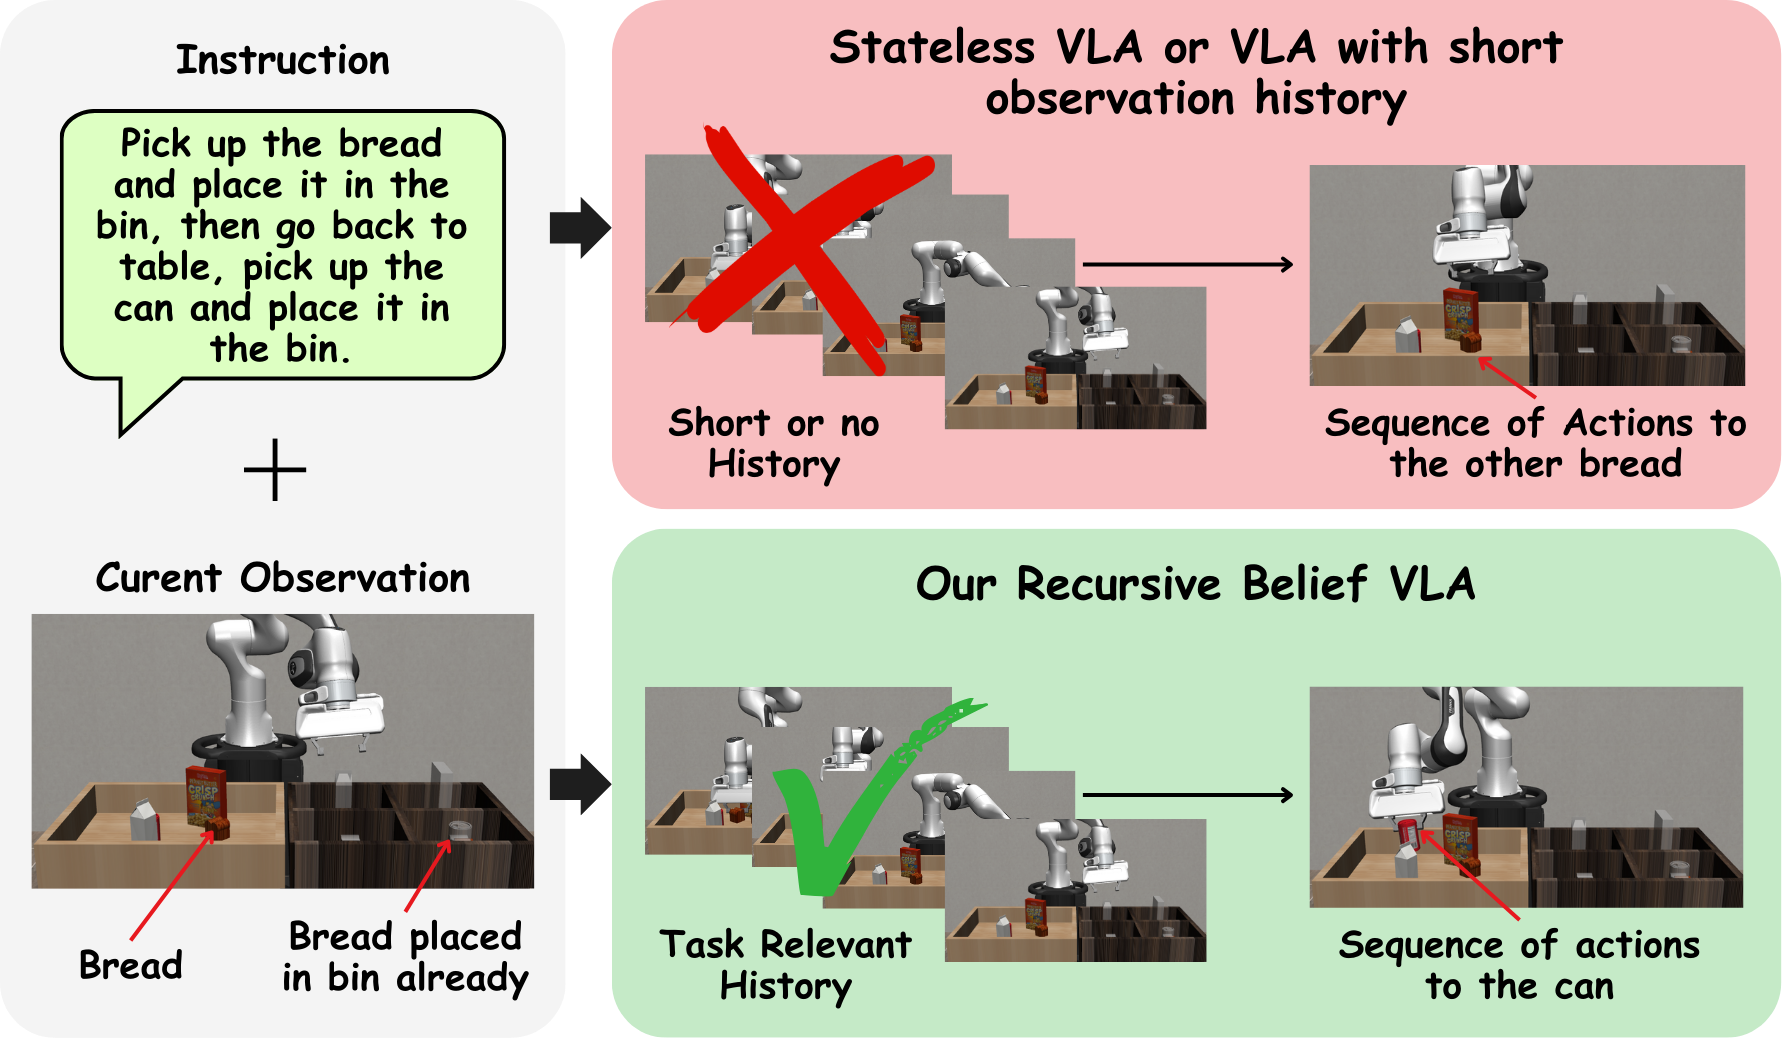
\includegraphics[width=0.7\textwidth, keepaspectratio]{belief_tokens.png}
\caption{Environment with similar objects.}
\label{fig:block1}
\end{figure}

Fig.~\ref{fig:block} illustrates how the intent embedding is obtained from the VLM. We remove the language generation head and use the frozen vision--language encoder to extract the final multi-modal hidden states. Let $X \in \mathbb{R}^{(T+V)\times D}$ denote the final multimodal hidden states of the VLM after fusion, where $T$ and $V$ correspond to language and visual tokens respectively, and $D$ is the hidden dimensionality. To extract an image-conditioned task representation, we apply a single-query attention pooling over these tokens. Specifically, we introduce a learned goal query vector $\mathbf{q} \in \mathbb{R}^{D}$ and compute
\begin{equation}
\alpha = \mathrm{softmax}\!\left(\frac{\mathbf{q}^\top W_k X^\top}{\sqrt{D}}\right),
\qquad
\mathbf{h}_{\text{task}} = \alpha X ,
\end{equation}
where $W_k$ is a learned projection matrix. The query $\mathbf{q}$ attends over the joint visual--linguistic token sequence and selectively pools tokens that are jointly grounded in the instruction and the initial scene. The result $\mathbf{h}_{\text{task}}$ is a single image-conditioned task vector that replaces the autoregressive language head with a compact, control-ready embedding. The pooled task vector is then projected through a lightweight MLP to obtain the intent vector $I_t$. The MLP adapts high-dimensional VLM features to the control space. The intent extraction module is trained end-to-end with the diffusion policy using the action prediction loss, while the VLM backbone remains frozen.

Figure~\ref{fig:block1} shows a multi-object manipulation task where short-horizon memory fails: once an object leaves view after being placed by the robot, stateless VLAs forget the interaction and reattempt grasping a similar object, while RB-VLA infers stage completion and continues the task.

\subsection{Low-Level Action Generation}
Low-level control is produced by a diffusion transformer policy that operates in latent space and is conditioned on the belief $b_t$, intent $I_t$, and a fused state representation $s_t$ from the state encoder. This encoder fuses robot proprioception and DINOv2 image embeddings to the same dimensions, decoupling multimodal perception from belief- and intent-level reasoning. The policy samples action chunks from
\begin{equation}
p\!\left(a_{t:t+H} \mid b_t, I_t, s_t \right) ,
\end{equation}
via iterative denoising, warm-started from the previously predicted action sequence with added low-variance Gaussian noise to improve sampling efficiency and temporal coherence. The diffusion model samples a chunk of $H$ actions jointly conditioned on the belief, intent, and fused state, allowing it to generate temporally coherent action sequences rather than independent per-step decisions. Warm-starting denoising from the previous chunk preserves smoothness across overlapping windows. Actions are executed in a receding-horizon manner at high frequency (50\,Hz), enabling smooth, closed-loop control under partial observability without reliance on dense semantic inference.

\subsection{Architecture and Implementation Details}
\label{subsec:arch}
This subsection summarises the concrete network configuration used for each module. Hidden dimensions are kept consistent at $d = 256$ across the belief, intent and policy stacks to simplify cross-module conditioning.

\paragraph{Visual backbone.} Visual observations are encoded by a frozen DINOv2 ViT-S/14 \cite{oquab2023dinov2} backbone, producing $16 \times 16 = 256$ patch tokens at 384 dimensions per frame. A linear projection maps these to the shared 256-dimensional space. Proprioceptive signals (end-effector pose, velocity, acceleration, force--torque) are embedded by a 2-layer MLP with hidden dimension 256 and GELU activations.

\paragraph{Frame fusion encoder.} The multimodal tokens of each frame are processed by a 4-block transformer encoder with 8 attention heads per block and feed-forward dimension $4d = 1024$. Pooling uses a single learnable query vector $d_q \in \mathbb{R}^{256}$, yielding the per-frame summary $f_t \in \mathbb{R}^{256}$.

\paragraph{Temporal transformer and recurrence.} Temporal integration is performed by a 4-block transformer (8 heads, FFN 1024) over a token sequence consisting of the previous belief token $b_{t-1}$ and the most recent $K = 5$ frame summaries. The output corresponding to the belief slot is treated as the evidence representation $e_t$. The deterministic belief recurrence is a single-layer GRU with hidden size 256 that integrates $e_t$ together with the stochastic latent $z_t$ to produce $b_t$.

\paragraph{Stochastic latent.} The prior $p(z_t \mid b_{t-1})$ and posterior $q(z_t \mid b_{t-1}, e_t)$ are diagonal Gaussians of dimension 32, predicted by 2-layer MLPs with hidden size 256 and reparameterised samples.

\paragraph{Predictive heads.} Both the one-step decoder and the auxiliary five-step decoder are 2-layer MLPs (hidden 512, GELU) producing 256-dimensional reconstructions in the EMA-frame-encoder feature space. The inverse-dynamics predictor $g(b_t, b_{t+1})$ is a 2-layer MLP (hidden 512) outputting actions in the same dimensionality as the robot action space.

\paragraph{Intent extractor.} The intent module attends over the final multi-modal hidden states of the frozen Qwen2.5-VL-7B \cite{bai2025qwen2} backbone (hidden size $D = 3584$). A learnable goal query $\mathbf{q} \in \mathbb{R}^{D}$ together with a key projection $W_k \in \mathbb{R}^{D \times D}$ yields the pooled task vector $\mathbf{h}_{\text{task}}$, which is mapped to a 256-dimensional intent $I_t$ by a 2-layer MLP. The VLM backbone is frozen; only the query, projection and MLP are trained.

\paragraph{Diffusion-transformer action head.} The DiT-based policy consists of 8 transformer blocks (8 heads, FFN 1024, hidden 256). Conditioning is provided via cross-attention on the concatenation $[b_t, I_t, s_t] \in \mathbb{R}^{768}$ together with sinusoidal embeddings of the diffusion timestep. The policy predicts a 16-step action chunk and is trained with the standard $\epsilon$-prediction objective using a cosine $\bar{\alpha}$ noise schedule over 100 DDPM steps.

\paragraph{Module sizes.} The belief stack (frame fusion, temporal transformer, GRU, stochastic head, predictive heads, inverse dynamics) totals approximately 150M parameters. The diffusion-transformer policy contains approximately 120M parameters. The frozen Qwen2.5-VL-7B backbone is shared across tasks and contributes no trainable parameters.

\section{Dataset and Training}
We use a staged training pipeline for the vision--language module, the belief model, and the diffusion controller. The belief transformer is first trained with the self-supervised objectives described in Section~\ref{subsec:belief}. The intent extraction layers and the diffusion policy are trained jointly. All models are trained using mixed precision and gradient accumulation.

\subsection{Dataset}
Training uses 40{,}000 simulated manipulation trajectories ($\sim$40M timesteps) across 10 tasks, collected in RoboSuite, LIBERO-Long, LIBERO-Object using Franka Panda and a UR5 MuJoCo environment. The dataset spans single and multi-object pick-and-place under occlusion, multi-block stacking in RoboSuite, and household tasks in LIBERO such as placing objects into drawers and cabinets. In practice, we observe that the belief converges reliably using a moderate number of trajectories, as the model focuses on learning control-relevant dynamics and action-conditioned state transitions rather than improving dense per-step semantic reasoning. We further finetune the belief and diffusion model with real-world manipulation tasks, adapting to sensor noise and unmodeled dynamics. During training, RGB observations are augmented with random brightness/contrast jitter, additive Gaussian noise, and minor spatial cropping to improve robustness and encourage learning of task-relevant state information.

\subsection{Training Details}
\label{subsec:training_details}
The belief model is trained first using the self-supervised objectives described in Section~\ref{subsec:belief}. The intent extraction module and the diffusion-transformer policy are then trained jointly with the action prediction loss while the VLM backbone and the trained belief encoder remain frozen. Refer to Section~\ref{subsec:arch} for the complete architectural configuration of each module. All experiments are run on 12 NVIDIA A100 GPUs (80\,GB) using distributed data parallel training with bfloat16 mixed precision and gradient accumulation. Total wall-clock training time is approximately 2.5 days for the belief model and 3 days for the diffusion policy.

\paragraph{Optimisation.} All learnable modules are optimised with AdamW ($\beta_1 = 0.9$, $\beta_2 = 0.95$, weight decay $0.05$). The peak learning rate of $1\times 10^{-4}$ is reached over a linear warm-up of $2{,}000$ steps and then decayed on a cosine schedule. Gradients are clipped to a global norm of $1.0$. Exponential moving averages (EMA) of the model weights are maintained with decay $0.999$ for the frame encoder used as a prediction target.

\paragraph{Loss balancing.} The multi-step prediction weight in Equation~(4) is set to $\lambda = 0.5$, balancing one-step and five-step ahead reconstruction. The KL coefficient $\beta$ is annealed linearly from $0$ to $10^{-3}$ over the first $10{,}000$ iterations of belief training and held constant thereafter, which we find sufficient to prevent posterior collapse without over-regularising the latent. The inverse-dynamics loss is added with weight $0.1$. The temporal contrastive warm-start objective uses a temperature of $0.07$ and treats frames within $\pm 5$ timesteps as positives.

\paragraph{Data augmentation.} During belief training, RGB observations are augmented with random brightness and contrast jitter ($\pm 0.2$), additive Gaussian noise ($\sigma = 0.02$), and random spatial crops of $0.9\times$--$1.0\times$ the image area, followed by resizing back to the network input resolution. Proprioceptive signals are perturbed with low-variance Gaussian noise to encourage robustness to sensor noise.

A summary of the principal training hyperparameters is given in Table~\ref{tab:hparams}, and the loss weights for the belief objective are listed in Table~\ref{tab:loss_weights}.

\begin{table}[h]
\centering
\caption{Principal training hyperparameters.}
\label{tab:hparams}
\begin{tabular}{lcc}
\toprule
\textbf{Setting} & \textbf{Belief Model} & \textbf{Diffusion Policy} \\
\midrule
Optimiser & AdamW & AdamW \\
$(\beta_1, \beta_2)$ & $(0.9, 0.95)$ & $(0.9, 0.95)$ \\
Weight decay & $0.05$ & $0.05$ \\
Peak learning rate & $1\times 10^{-4}$ & $1\times 10^{-4}$ \\
LR schedule & cosine, $2$k warm-up & cosine, $2$k warm-up \\
Gradient clip (global $\ell_2$) & $1.0$ & $1.0$ \\
Effective batch size & $128$ & $32$ \\
Iterations & $80{,}000$ & $100{,}000$ \\
Precision & bf16 mixed & bf16 mixed \\
Hardware & $12\times$A100 80\,GB & $12\times$A100 80\,GB \\
\bottomrule
\end{tabular}
\end{table}

\begin{table}[h]
\centering
\caption{Loss weights used in belief-model training (Equation~(4) and inverse-dynamics objective).}
\label{tab:loss_weights}
\begin{tabular}{lc}
\toprule
\textbf{Term} & \textbf{Weight} \\
\midrule
Next-frame reconstruction $\log p(x_{t+1} \mid b_t, z_t)$ & $1.0$ \\
Multi-step reconstruction weight $\lambda$ on $x_{t+5}$ & $0.5$ \\
KL coefficient $\beta$ (annealed) & $0 \rightarrow 10^{-3}$ over 10k iters \\
Inverse-dynamics $\mathcal{L}_{\text{inv}}$ & $0.1$ \\
Temporal contrastive (warm-start) & $1.0$ \\
\bottomrule
\end{tabular}
\end{table}

\section{Results}
Recursive Belief VLA (RB-VLA) is evaluated in simulation and the real world, using RoboSuite and LIBERO-Long. The evaluation focuses on: (a) long-horizon tasks; (b) latency and memory growth; (c) belief representation analysis; (d) ablation studies; (e) real world tasks. Before presenting results, Section~\ref{subsec:exp_setup} consolidates the evaluation protocol, baselines, metrics and hardware used across all experiments.

\subsection{Experimental Setup}
\label{subsec:exp_setup}

\paragraph{Tasks and environments.} RB-VLA is evaluated in three settings. \textit{(i)} Long-horizon, multi-stage manipulation in RoboSuite using a Franka Panda manipulator, focusing on multi-object pick-and-place and multi-block stacking under both clean and partially observed conditions. \textit{(ii)} Household manipulation in LIBERO-Long, including drawer and cabinet interactions that require sustained task tracking across many timesteps. \textit{(iii)} Real-world manipulation on a UR5 manipulator with an Intel RealSense D435i RGB camera, using objects of varying colours and shapes placed in randomised configurations. Tasks in all three settings are specified by a natural language instruction supplied at $t=0$.

\paragraph{Baselines.} RB-VLA is compared against three representative VLA architectures spanning the dominant design choices in the literature: \textbf{OpenVLA} \cite{kim2024openvla}, a stateless autoregressive token-based model; \textbf{GR00T-N1} \cite{bjorck2025gr00t}, a multi-frame VLA with a diffusion-based controller; and \textbf{$\pi_0$} \cite{black2025pi_}, a flow-matching policy with strong reported long-horizon performance. For fair comparison, every baseline is fine-tuned on the same 40k-trajectory simulation dataset using its official training procedure, and is evaluated on the same task instances as RB-VLA.

\paragraph{Metrics.} We report three primary metrics. The \textbf{task success rate} is the fraction of evaluation episodes that complete the target task within a fixed time budget without collision, premature termination, or constraint violation. The \textbf{inference latency} is the average end-to-end wall-clock time per action chunk on a single NVIDIA A100 GPU, reported as the per-episode mean. The \textbf{relative memory usage} is reported as a multiple of the single-frame baseline, isolating the architectural memory growth induced by additional temporal context.

\paragraph{Evaluation protocol.} Every reported simulation success rate is averaged over $40$ trials per task with different random seeds. Robustness is stress-tested at inference by randomising object identities and placements, environment configurations, lighting conditions, object presentation order, and by introducing dropped frames and additive observation noise. Real-world results are averaged over $25$ trials per task with hand-randomised object placements, with no resets or human intervention permitted during a trial. Models are always evaluated on held-out task instances that are not encountered during training.

\paragraph{Hardware.} Training is performed on $12\times$ NVIDIA A100 80\,GB GPUs with distributed data-parallel training (Section~\ref{subsec:training_details}). Inference benchmarks (latency and memory) are conducted on a single A100. For real-world deployment, the UR5 controller runs at $50$\,Hz, the diffusion policy samples action chunks at $10$--$20$\,Hz, and the recursive belief is updated at the same rate as new observations arrive.

\subsection{Long Horizon Tasks}
We evaluate RB-VLA on long-horizon, multi-stage manipulation tasks with and without occlusion, assessing robustness under partial observability as well as sustained task progression over extended horizons. Experiments follow the protocol of Section~\ref{subsec:exp_setup}, with 40 trials per task. Quantitative results for two-object pick-and-place under occlusion and for stacking are reported in Table~\ref{tab:longhorizon}.

\begin{table}[h]
\centering
\caption{Long-horizon success rates (\%) for pick-and-place (P\&P) and stacking tasks.}
\label{tab:longhorizon}
\begin{tabular}{lcccc}
\hline
Method & Single P\&P & Multi P\&P & Single Stack & Multi Stack \\
\hline
GROOT-N1 & 52.5 & 20.0 & 67.5 & 40.0 \\
OpenVLA & 22.5 & $\times$ & $\times$ & $\times$ \\
$\pi_0$ & 55.0 & 25.0 & 70.0 & 47.5 \\
RB-VLA (ours) & \textbf{82.5} & \textbf{77.5} & \textbf{85.0} & \textbf{80.0} \\
\hline
\end{tabular}
\end{table}

RB-VLA achieves substantially higher performance across all long-horizon tasks, exceeding $\pi_0$ by 52.5\% and GROOT-N1 by 57.5\% on multi-stage pick-and-place under partial observability, while OpenVLA fails to complete the task in this setting. These baselines repeatedly invoke VLMs for step-wise semantic reasoning, but lack awareness of task progression in multi-stage tasks and lose object or state awareness under occlusion. Belief-based models address this limitation by capturing temporal dynamics and enabling causal reasoning, whereas VLMs are primarily used for semantic inference. This demonstrates that belief-based state estimation is crucial for robust long-horizon, multi-stage control.

Figure~\ref{fig:motion} illustrates representative multi-stage executions in which earlier object interactions become occluded. The learned belief state preserves the necessary context to disambiguate visually similar objects and maintain consistent task progression.

\begin{figure}[!htbp]
\centering
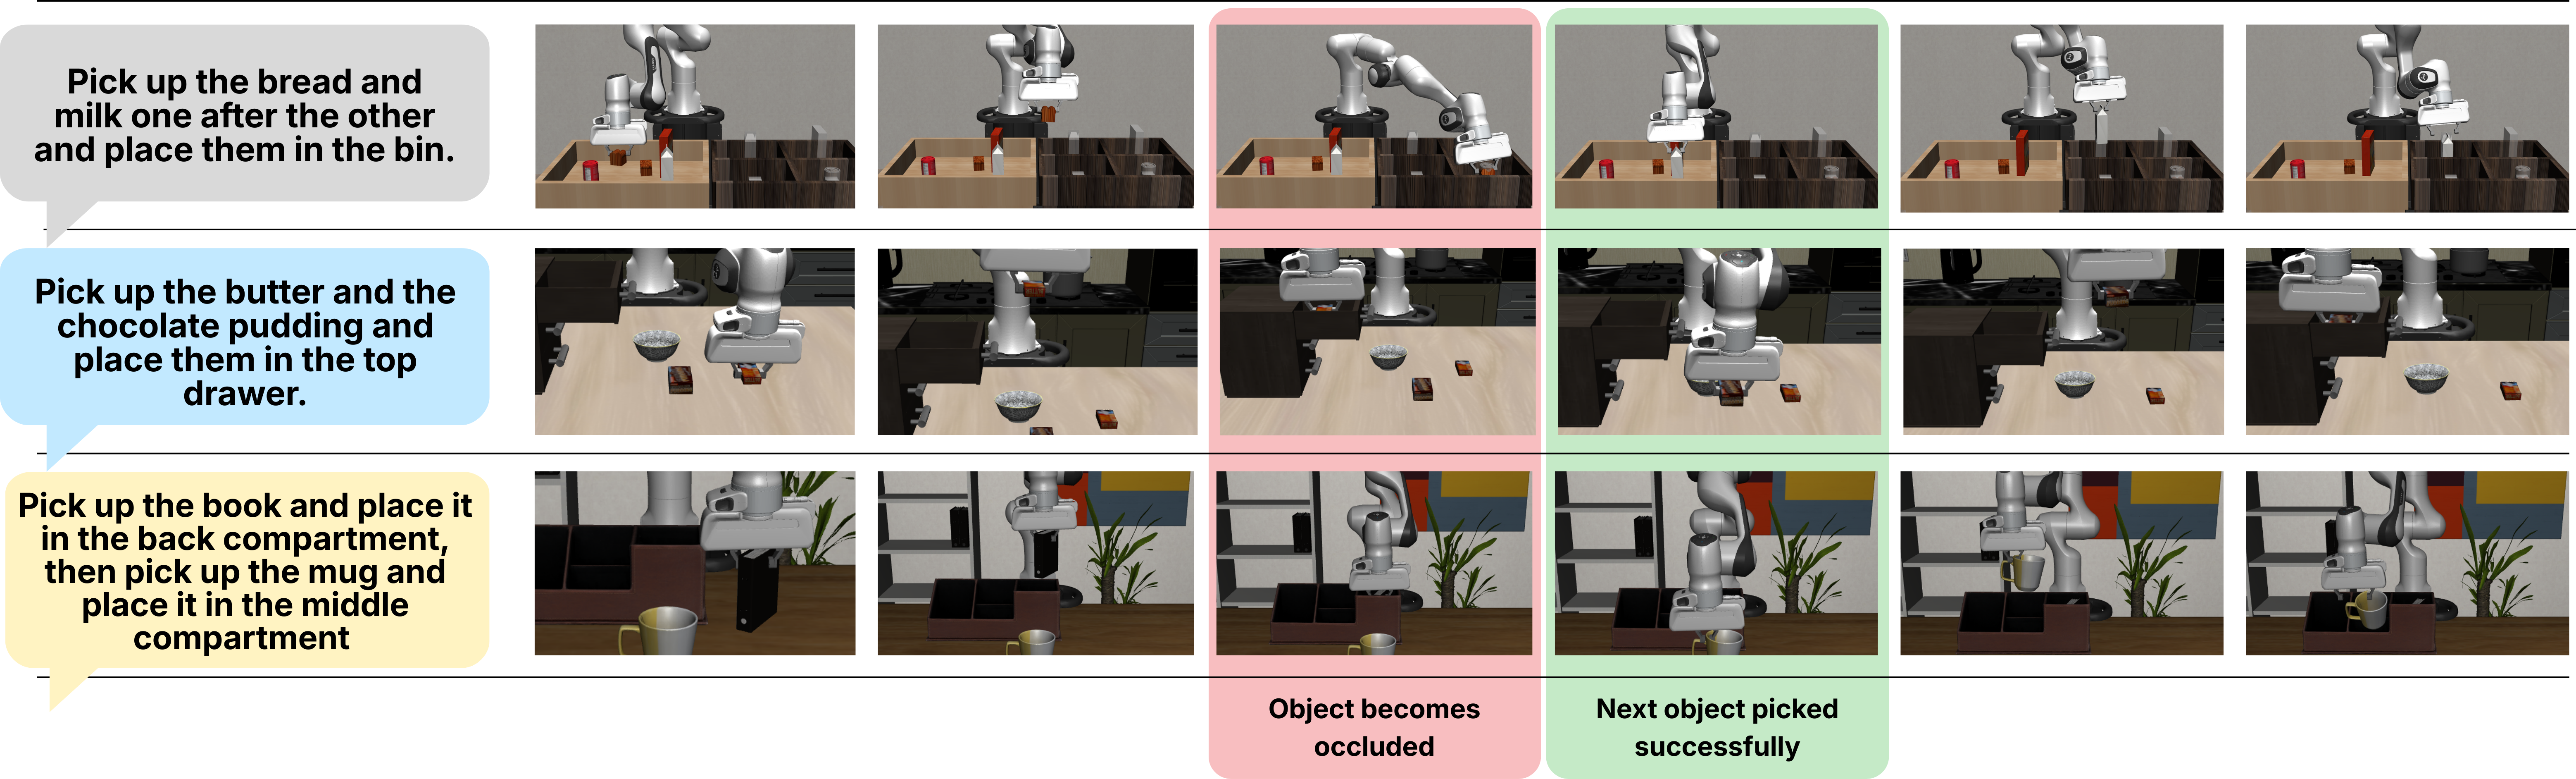
\includegraphics[width=\textwidth, keepaspectratio]{motion1.png}
\caption{\textbf{Long-horizon tasks under partial observability}. After the first object is placed and becomes occluded, the model correctly selects the subsequent target despite visually similar objects, avoiding re-grasping the same object.}
\label{fig:motion}
\end{figure}

\subsection{Latency and Memory Analysis}
We evaluate computational efficiency using latency and memory, with all inference measurements performed on one NVIDIA A100 GPU. Figure~\ref{fig:latency} compares the average episode latency of RB-VLA with prior methods. Since task instructions and semantic goals remain fixed within an episode, RB-VLA queries the VLM only once at the beginning of the task to obtain the intent embedding, and does not re-invoke it during execution. As a result, RB-VLA achieves over five times lower latency than stateless OpenVLA and RT1-X, and is more than three times faster than multi-frame GR00T-N1, which repeatedly processes multiple visual frames. This demonstrates that decoupling semantic grounding from control enables efficient real-time deployment.

\begin{figure}[h]
\centering
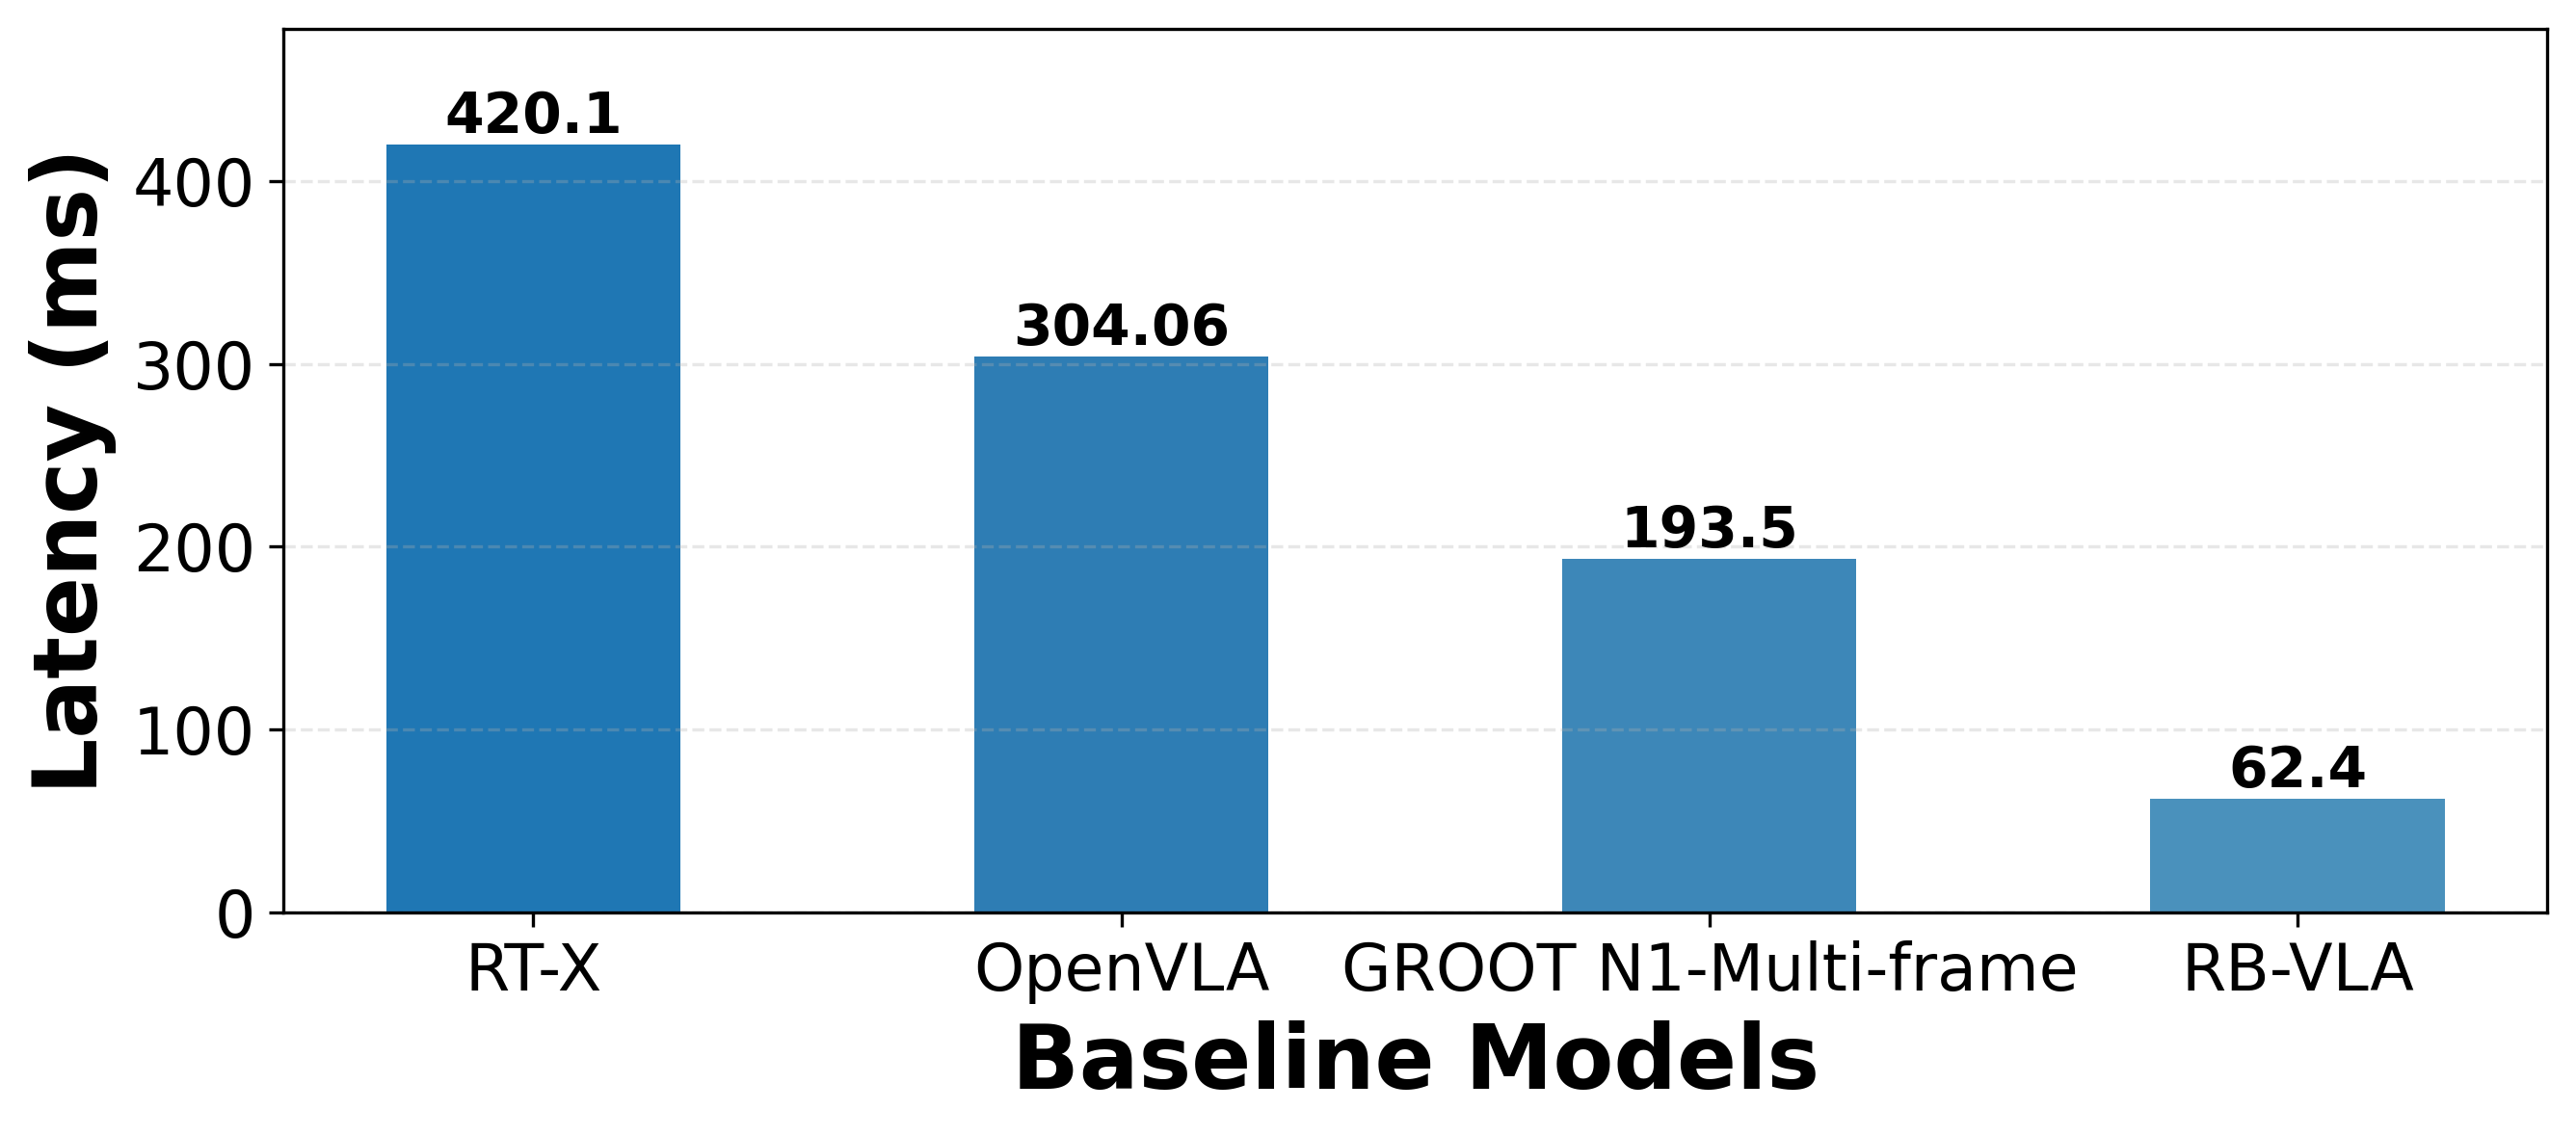
\includegraphics[width=0.7\textwidth, keepaspectratio]{latency_comparison.png}
\caption{Average inference latency per episode for RB-VLA and baseline VLA methods.}
\label{fig:latency}
\end{figure}

Many VLA systems maintain temporal context by accumulating multiple past frames or memory tokens, causing memory and compute to scale with interaction horizon. Table~\ref{tab:memory_scaling} shows that both large VLM backbones (Qwen2-VL-7B) and end-to-end VLA systems (GR00T-N1) exhibit superlinear memory growth as the number of observed frames increases. In contrast, RB-VLA recursively compresses all task-relevant interaction history into a fixed-size belief state, yielding constant memory usage independent of episode length and enabling scalable long-horizon control.

\begin{table}[h]
\centering
\renewcommand{\arraystretch}{1.2}
\caption{Relative memory usage as a function of temporal context length, comparing RB-VLA with baseline models.}
\label{tab:memory_scaling}
\begin{tabular}{lccc}
\toprule
\textbf{Temporal Context} & \textbf{Qwen2-VL-7B} & \textbf{GR00T-N1} & \textbf{RB-VLA (Ours)} \\
\midrule
1 frame  & $1.00\times$  & $1.00\times$  & $1.0\times$ \\
2 frames  & $1.81\times$ & $2.21\times$  & $1.0\times$ \\
4 frames  & $3.64\times$ & $3.85\times$ & $1.0\times$ \\
8 frames  & $6.82\times$  & $7.12\times$  & $1.0\times$ \\
\bottomrule
\end{tabular}
\end{table}

\subsection{Belief Representation Analysis}
We evaluate belief quality by sampling pairs of belief states and testing whether proximity in belief space predicts similarity in future dynamics and control behaviour. For each pair, we compute cosine similarity between their belief representations and compare it to (i) the norm of the distance between the corresponding future action sequences and (ii) the cosine similarity between their future visual feature representations. Unlike stage-labelled analysis with discrete phases (e.g., grasp, transport, place), manipulation dynamics evolve smoothly, thus belief quality is reflected in predictive consistency rather than phase separability.

As shown in Fig.~\ref{fig:belief_similarity}, belief similarity exhibits a strong monotonic relationship with both future visual similarity (Pearson $r=0.78$) and future action similarity ($r=0.87$). The shaded red region represents the variance, with $\sigma_{\text{bottom }20\%} = 2.3\,\sigma_{\text{top }20\%}$, indicating that similar beliefs encode consistent underlying dynamics and lead to similar action outcomes and future observations, while dissimilar beliefs correspond to different dynamical regimes, admitting multiple plausible future trajectories. This provides evidence that the belief acts as a latent action-conditioned dynamical state, governing future closed-loop evolution under control.

To analyse stochasticity, we fix a belief state $b_t$ and sample multiple latent variables $z_t \sim p(z_t \mid b_t)$. Figure~\ref{fig:stochasticity} shows that different latent samples produce diverse yet structured future predictions, indicating that the belief encodes sharp underlying dynamics while $z_t$ captures uncertainty and multimodality over plausible future evolutions. The KL divergence stabilises at a non-zero value, indicating sustained usage of $z_t$ and preventing collapse to a single averaged future. These results demonstrate that the belief filters perceptual noise and preserves control-relevant structure.

\begin{figure}[h]
    \centering
    \begin{subfigure}{\linewidth}
        \centering
        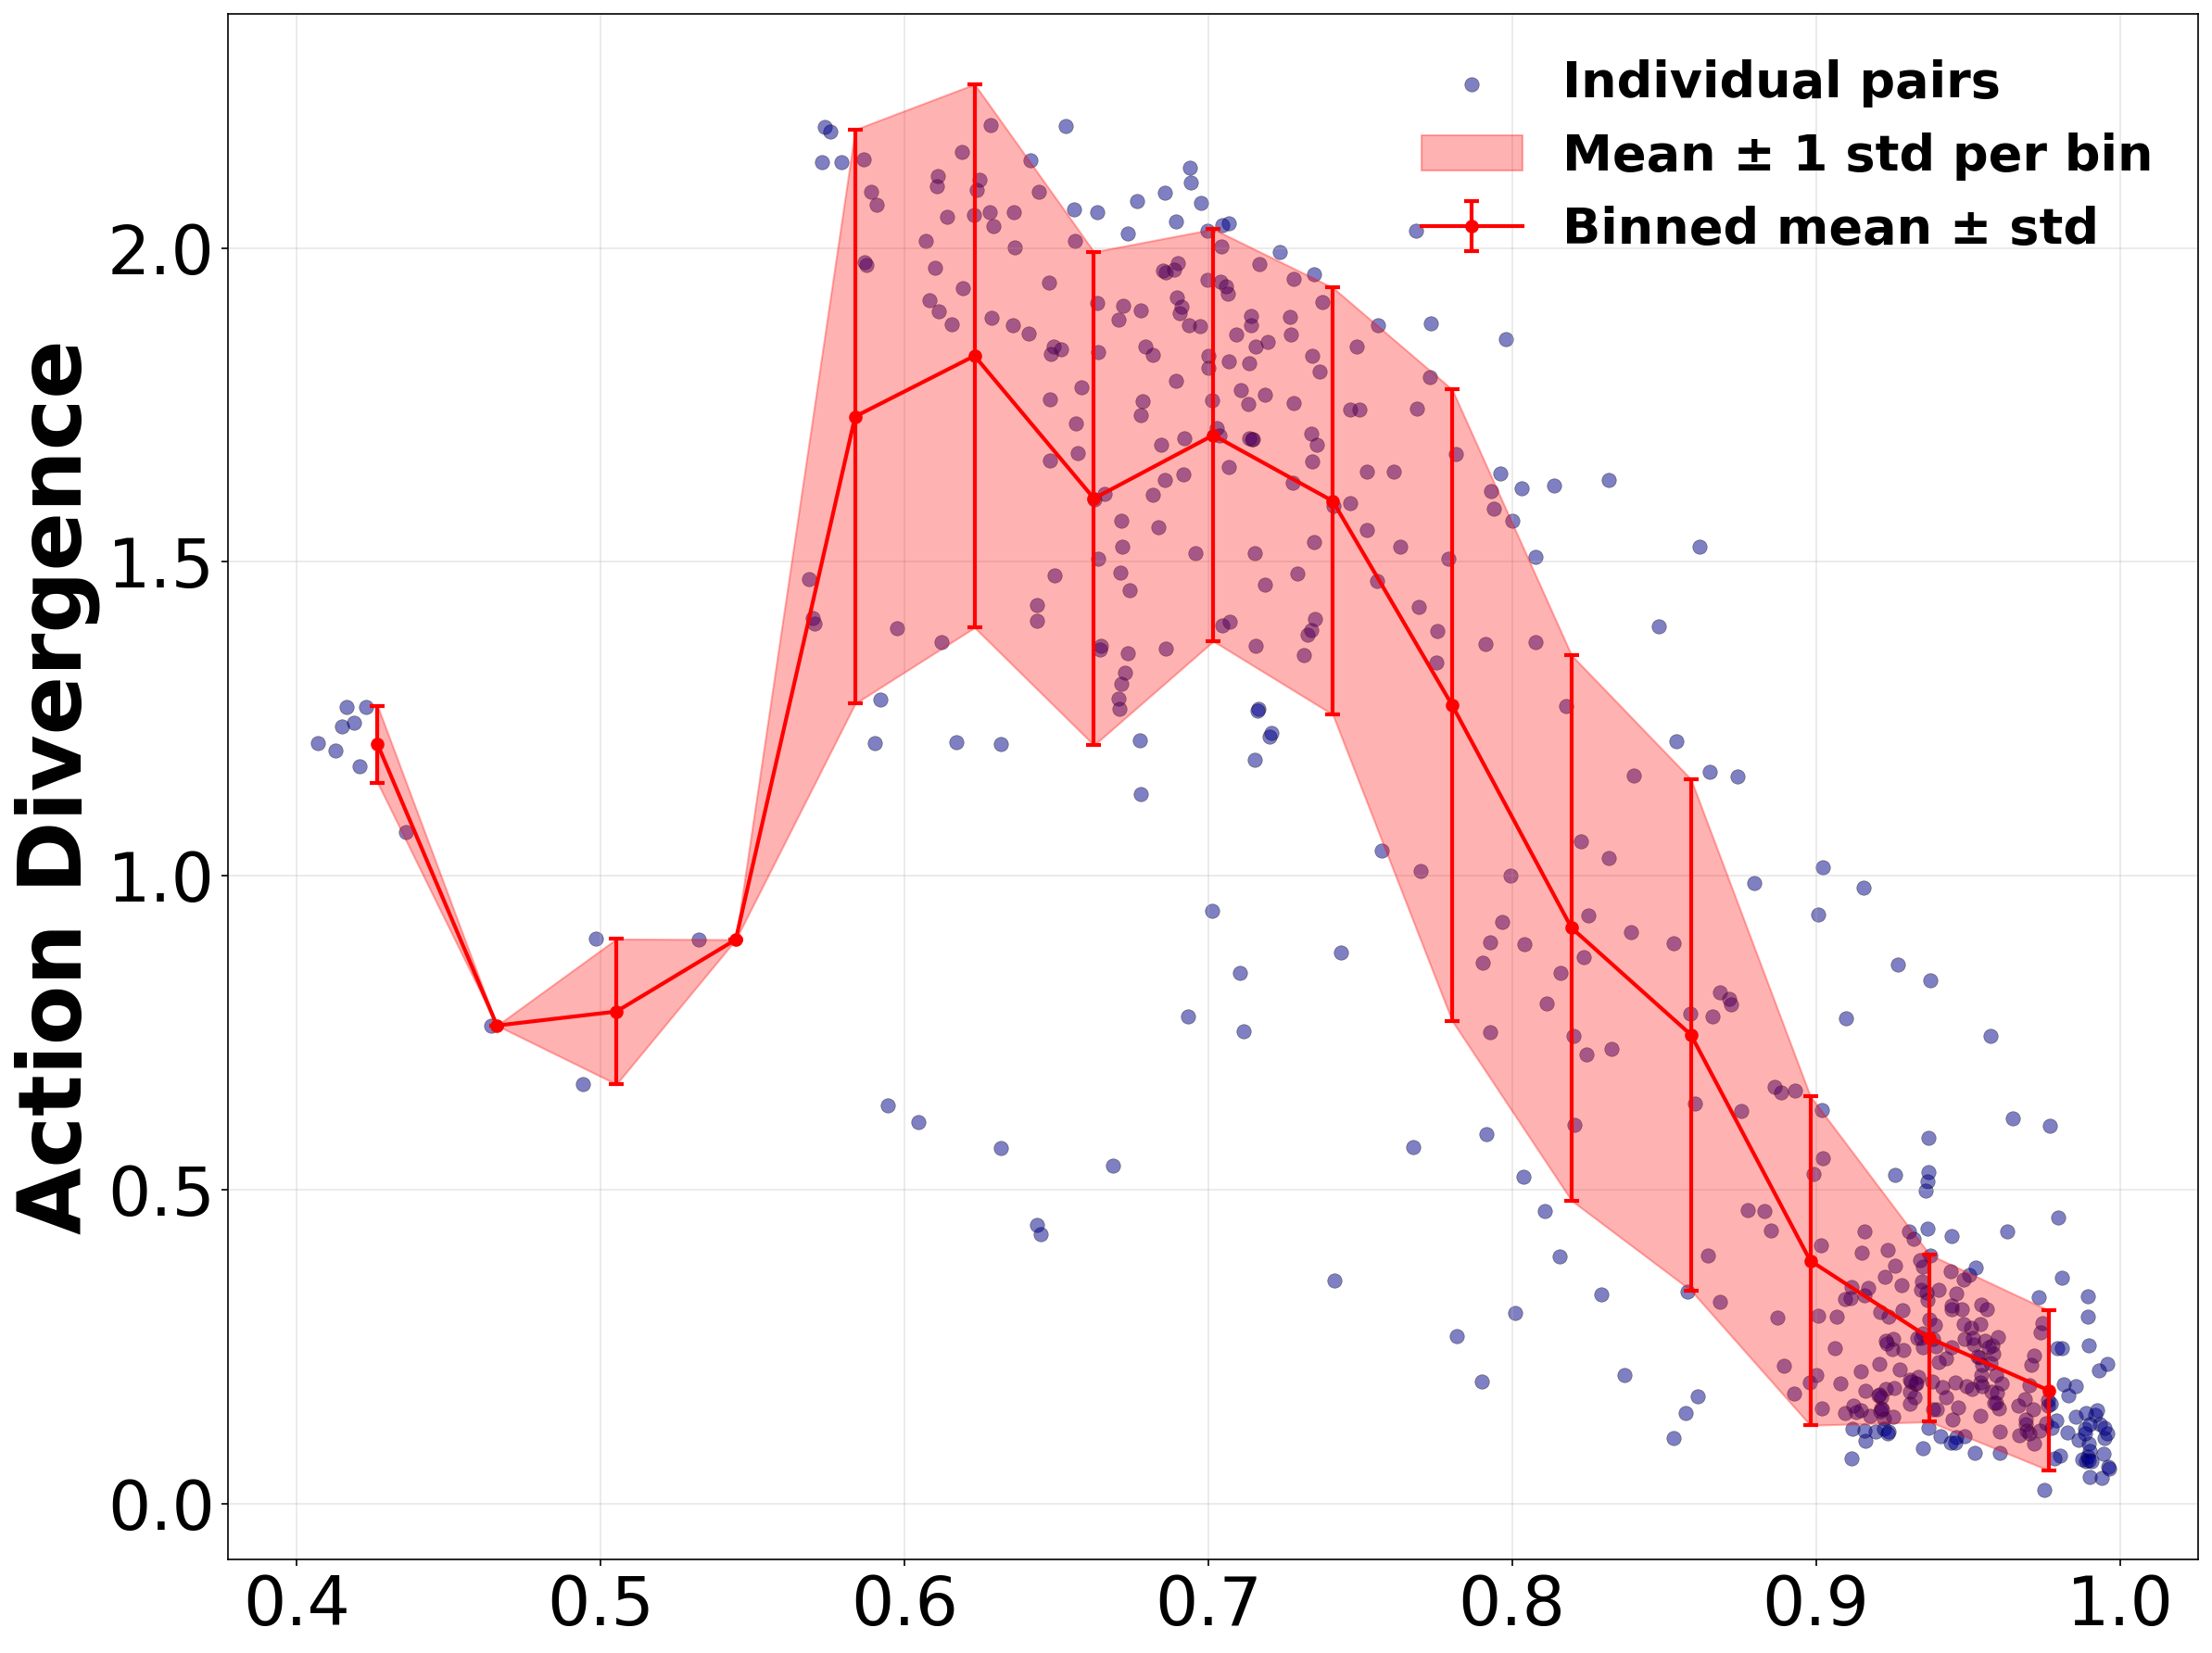
\includegraphics[height=0.18\textheight]{action.png}
    \end{subfigure}
    \vspace{4pt}
    \begin{subfigure}{\linewidth}
        \centering
        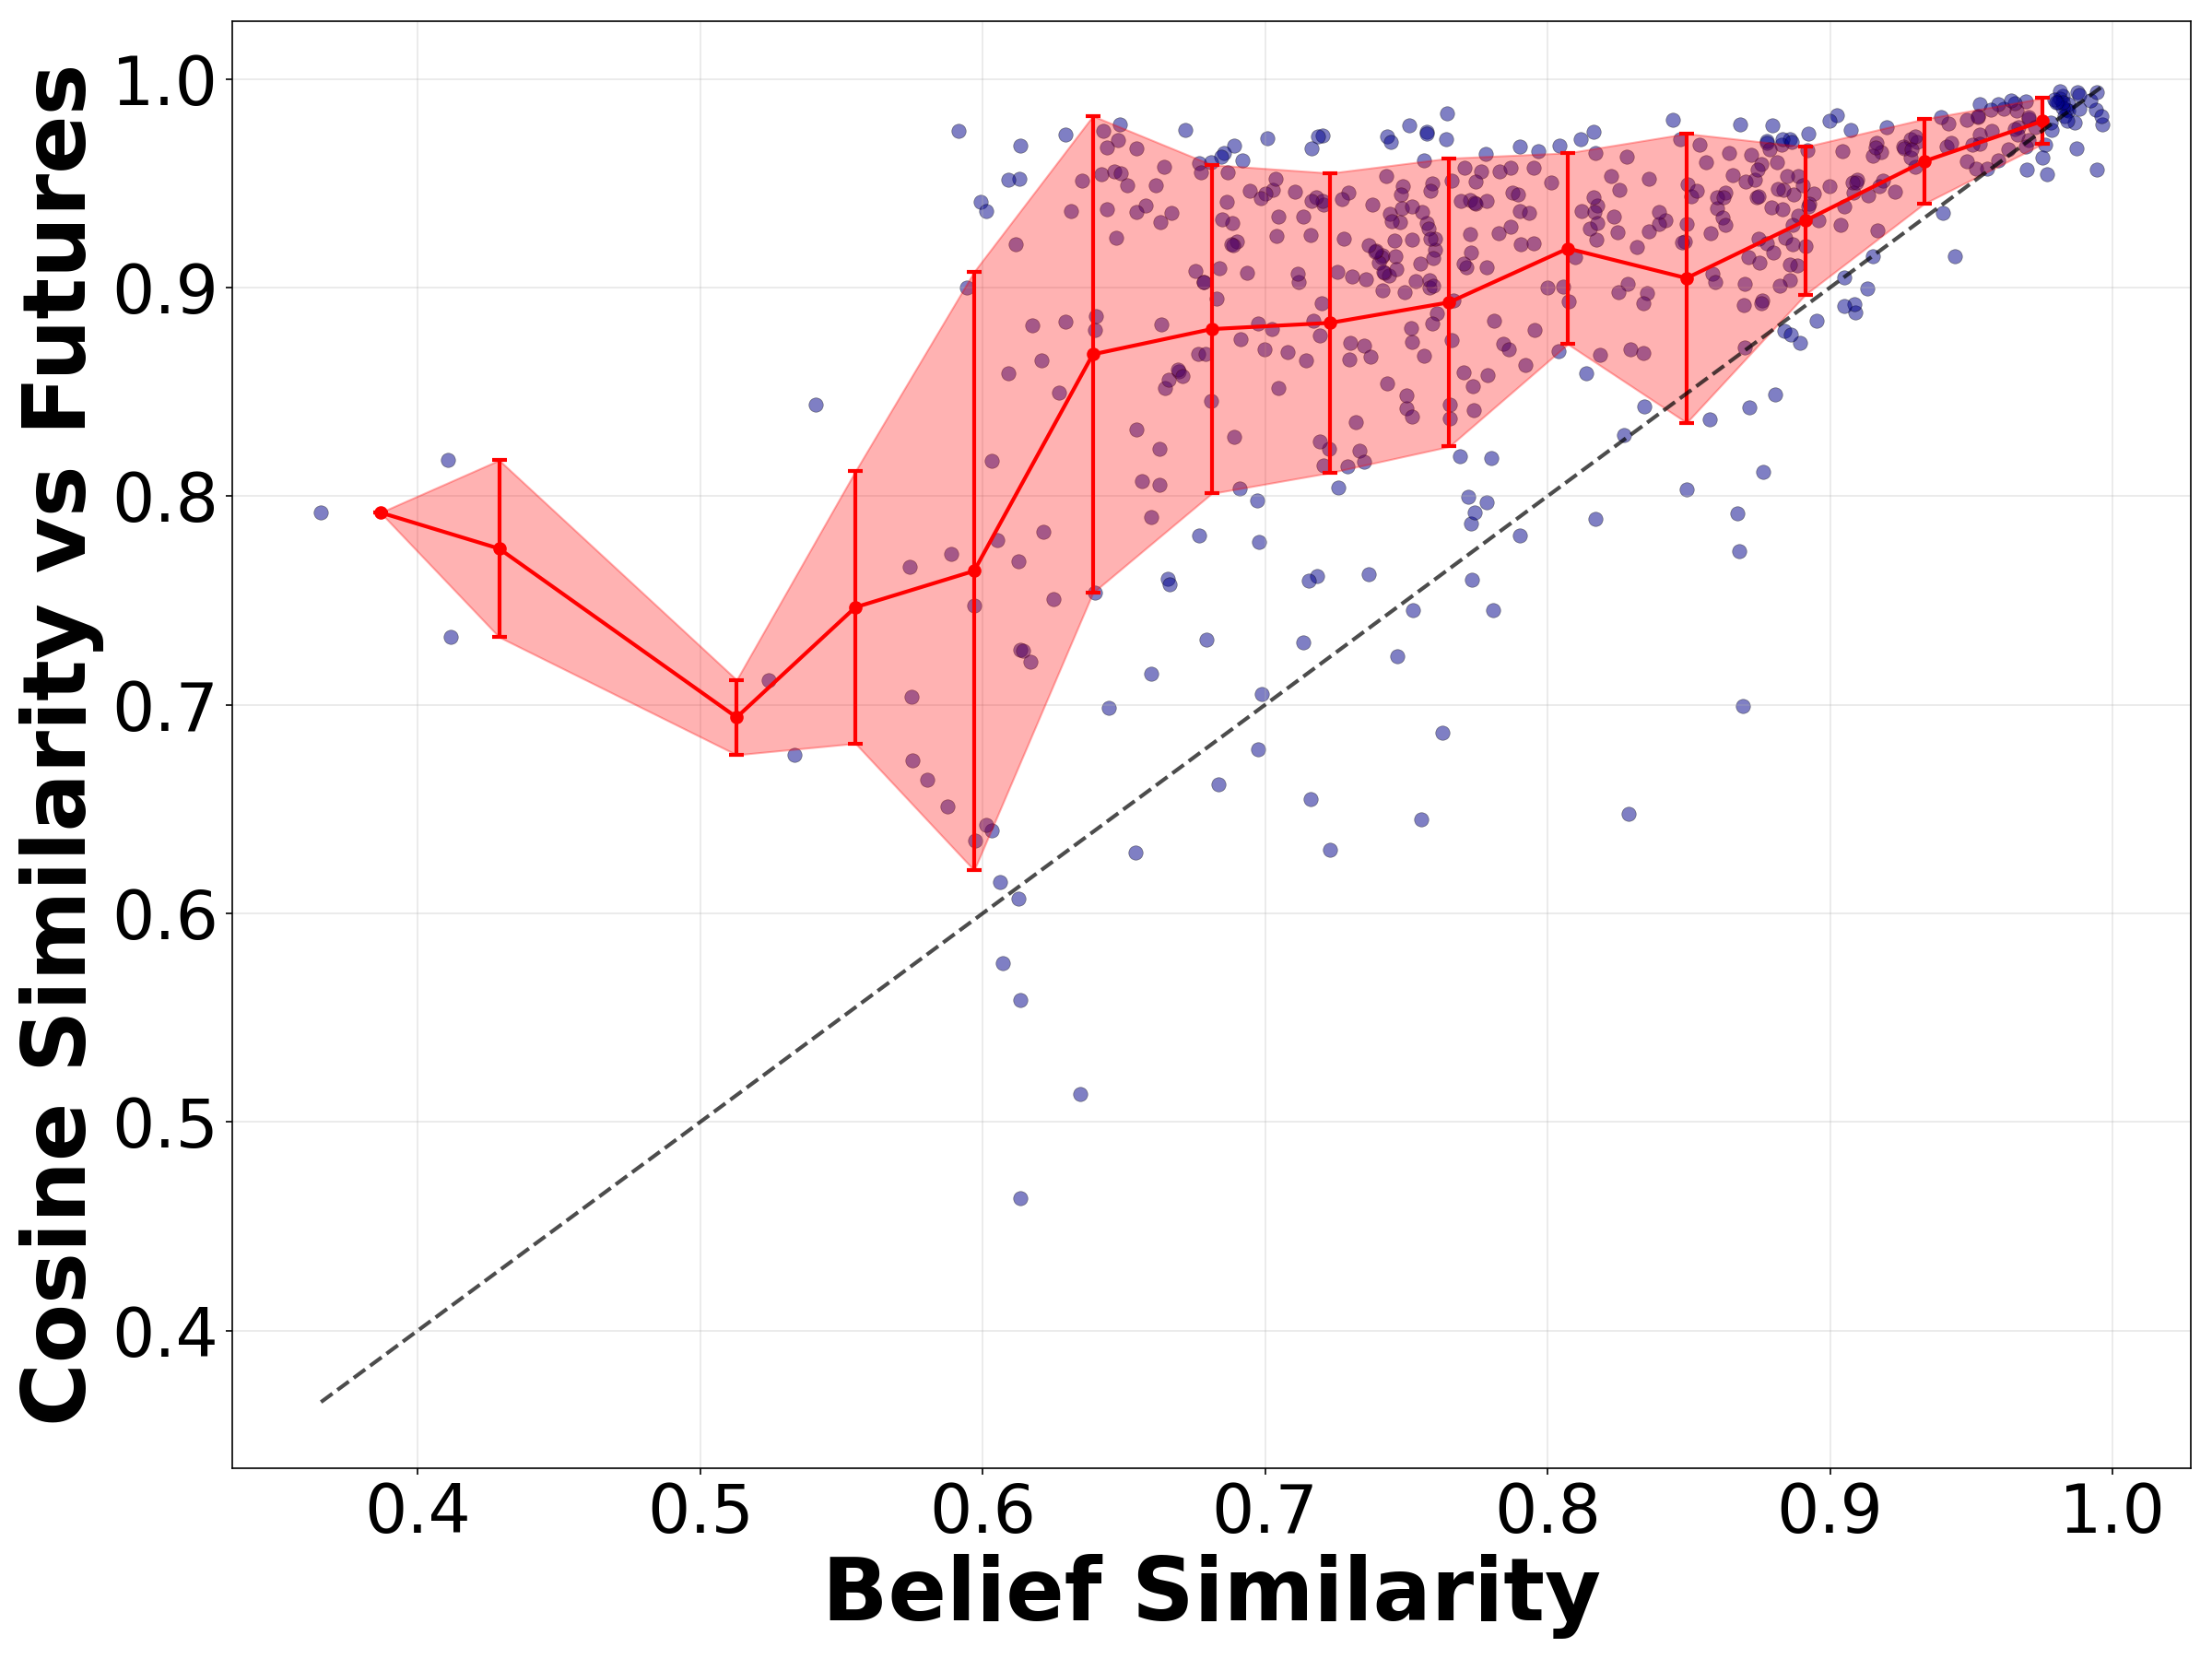
\includegraphics[height=0.18\textheight]{future.png}
    \end{subfigure}
    \caption{(a) Future action divergence versus belief cosine similarity. (b) Future observation cosine similarity versus belief cosine similarity. Both plots exhibit strong monotonic correlation, indicating that proximity in belief space predicts similarity in future perception and control behaviour.}
    \label{fig:belief_similarity}
\end{figure}

\begin{figure}[h]
    \centering
    \begin{subfigure}{\linewidth}
        \centering
        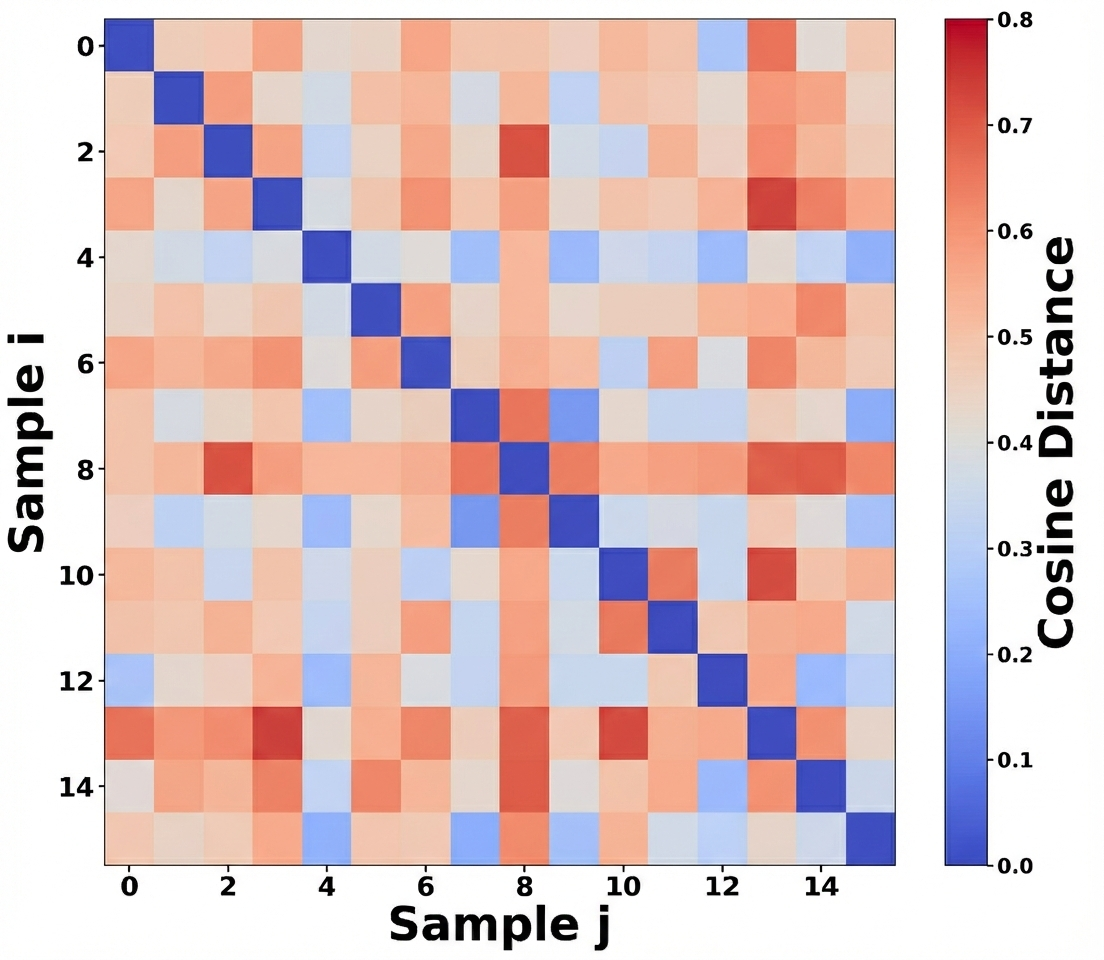
\includegraphics[height=0.27\textheight]{div2.png}
    \end{subfigure}
    \vspace{8pt}
    \begin{subfigure}{\linewidth}
        \centering
        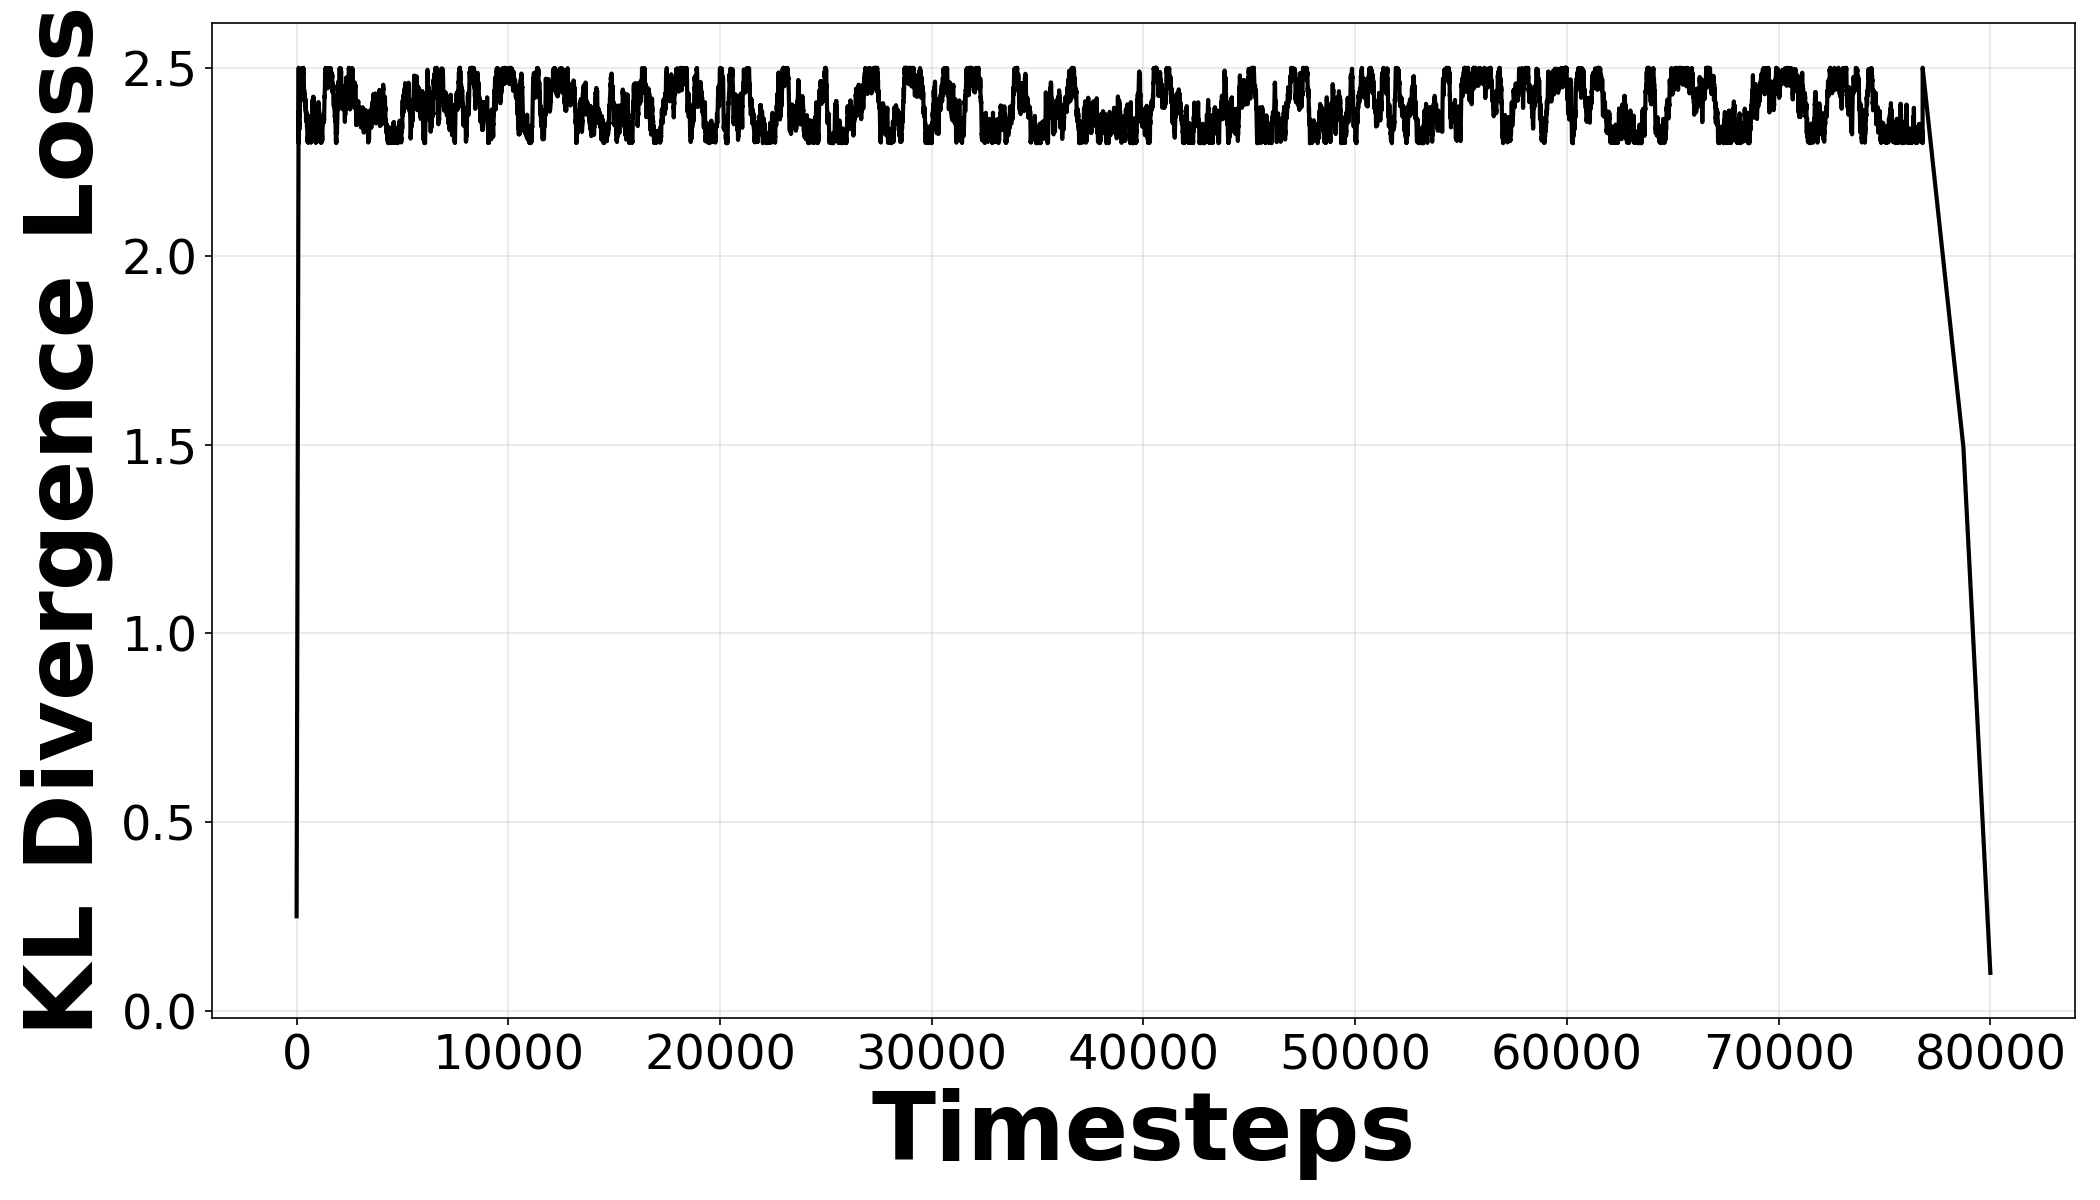
\includegraphics[height=0.18\textheight]{kl_losses_training.png}
    \end{subfigure}
    \caption{(i) Future divergence using cosine distance with multiple sampled latent variables ($n=16$) from a fixed belief state $b_t$, illustrating stochastic rollout diversity. (ii) KL divergence loss across training, showing stable convergence of the belief model's latent distribution.}
    \label{fig:stochasticity}
\end{figure}

Figure~\ref{fig:attention} visualises attention weights at timesteps where the manipulated object becomes occluded. The belief attends to its recursive state and causally informative past frames, adaptively retaining relevant dynamical history while discarding irrelevant information for future prediction.

\begin{figure}[h]
\centering
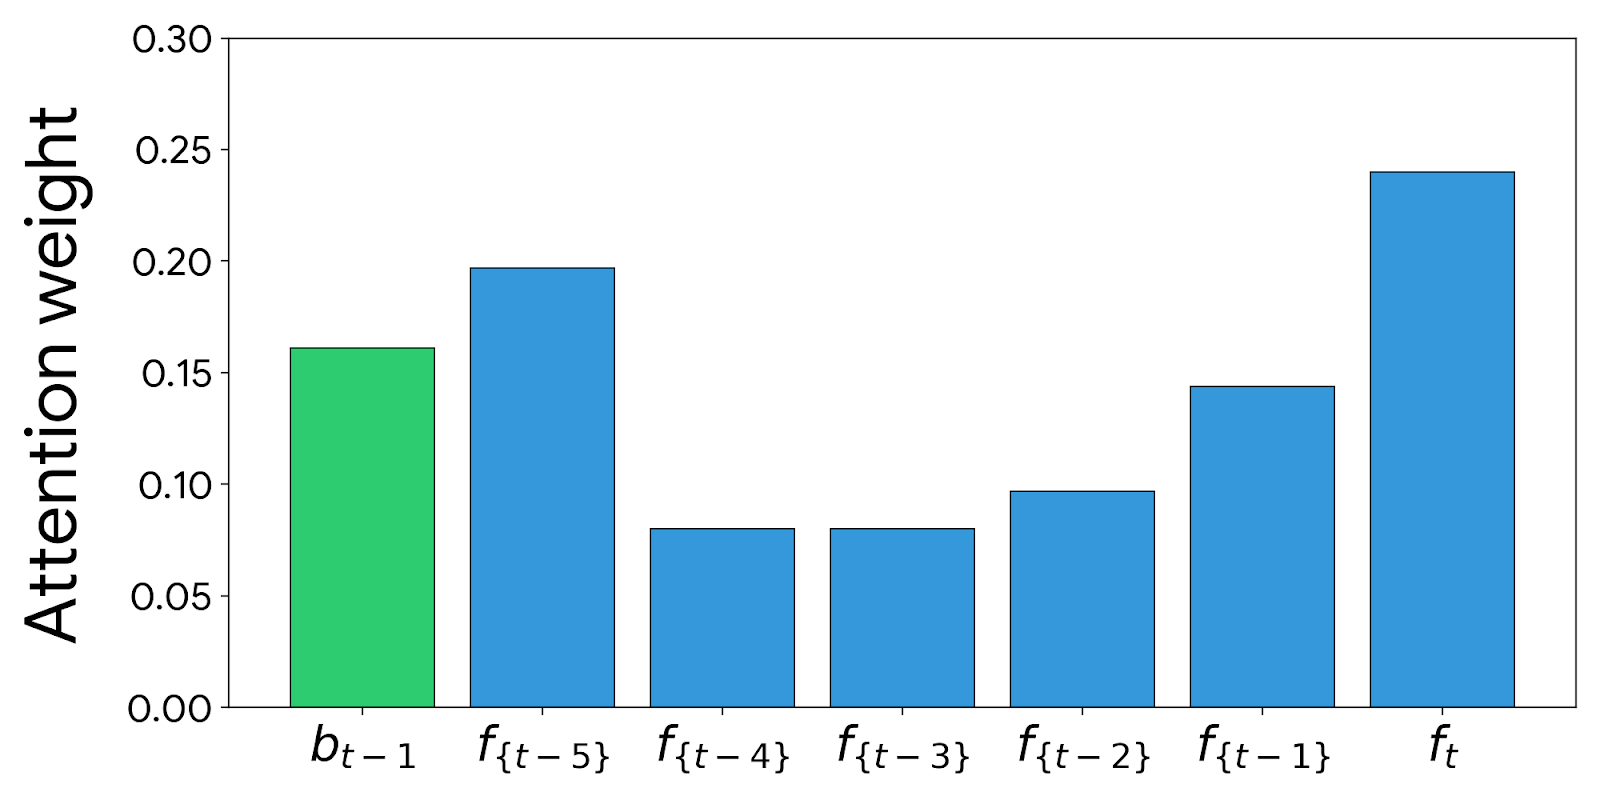
\includegraphics[width=0.7\textwidth, keepaspectratio]{att_weights.png}
\caption{Normalised self-attention weights of the temporal transformer over the previous recursive belief token and short history of input frame encoder tokens, indicating which tokens contribute to the belief state at time $t$.}
\label{fig:attention}
\end{figure}

\subsection{Ablation Study}
We ablate key components by selectively removing them and measuring the drop in average success rate over 40 episodes on the same long-horizon, multi-stage tasks under partial observability. Starting from the full RB-VLA, we evaluate: (i) no frame-encoder targets for training the belief (using only vision embeddings), (ii) deterministic belief without stochastic latent variables, and (iii) no belief--policy conditioning. As shown in Table~\ref{tab:ablation}, each removal degrades performance, with the lowest performance when belief is decoupled from control (a standard DiT policy) and the highest success achieved by the full RB-VLA. This highlights the need for a dynamics-grounded belief state, since the diffusion model alone lacks the dynamics-consistent causal state required for long-horizon, multi-stage behaviour.

\begin{table}[h]
\centering
\caption{Component ablation on two-object pick-and-place task. Average success rate over 40 episodes under partial observability.}
\label{tab:ablation}
\setlength{\tabcolsep}{6pt}
\renewcommand{\arraystretch}{1.0}
\begin{tabular}{cccc}
\toprule
\textbf{Frame Encoder} & \textbf{Stoch.\ $z$} & \textbf{Belief$\rightarrow$Policy} & \textbf{Success} \\
\midrule
$\times$ & $\times$ & $\times$ & 32.5 \\
$\times$ & $\times$ & $\checkmark$ & 57.5 \\
$\times$ & $\checkmark$ & $\checkmark$ & 62.5 \\
$\checkmark$ & $\checkmark$ & $\checkmark$ & \textbf{77.5} \\
\bottomrule
\end{tabular}
\end{table}

\subsection{Real World Deployment}
We deploy RB-VLA on a physical UR5 manipulator under conditions closely matching the UR5 MuJoCo setup used in simulation. The model successfully transfers to real hardware without architectural changes, demonstrating effective sim-to-real transfer. The diffusion policy is further fine-tuned on 100 real-world trajectories to adapt to sensor noise and unmodeled dynamics. Using the learned belief representation, the system achieves reliable long-horizon execution on multi-object pick-and-place tasks under partial observability, maintaining low inference latency and stable closed-loop control despite visual noise and actuation variability. After placement, the first object becomes fully occluded and is no longer visible in the camera view. Over 25 real-world trials, RB-VLA achieves a 68.0\% success rate, successfully completing grasp--transport--place cycles without manual intervention.

\begin{figure}[h]
\centering
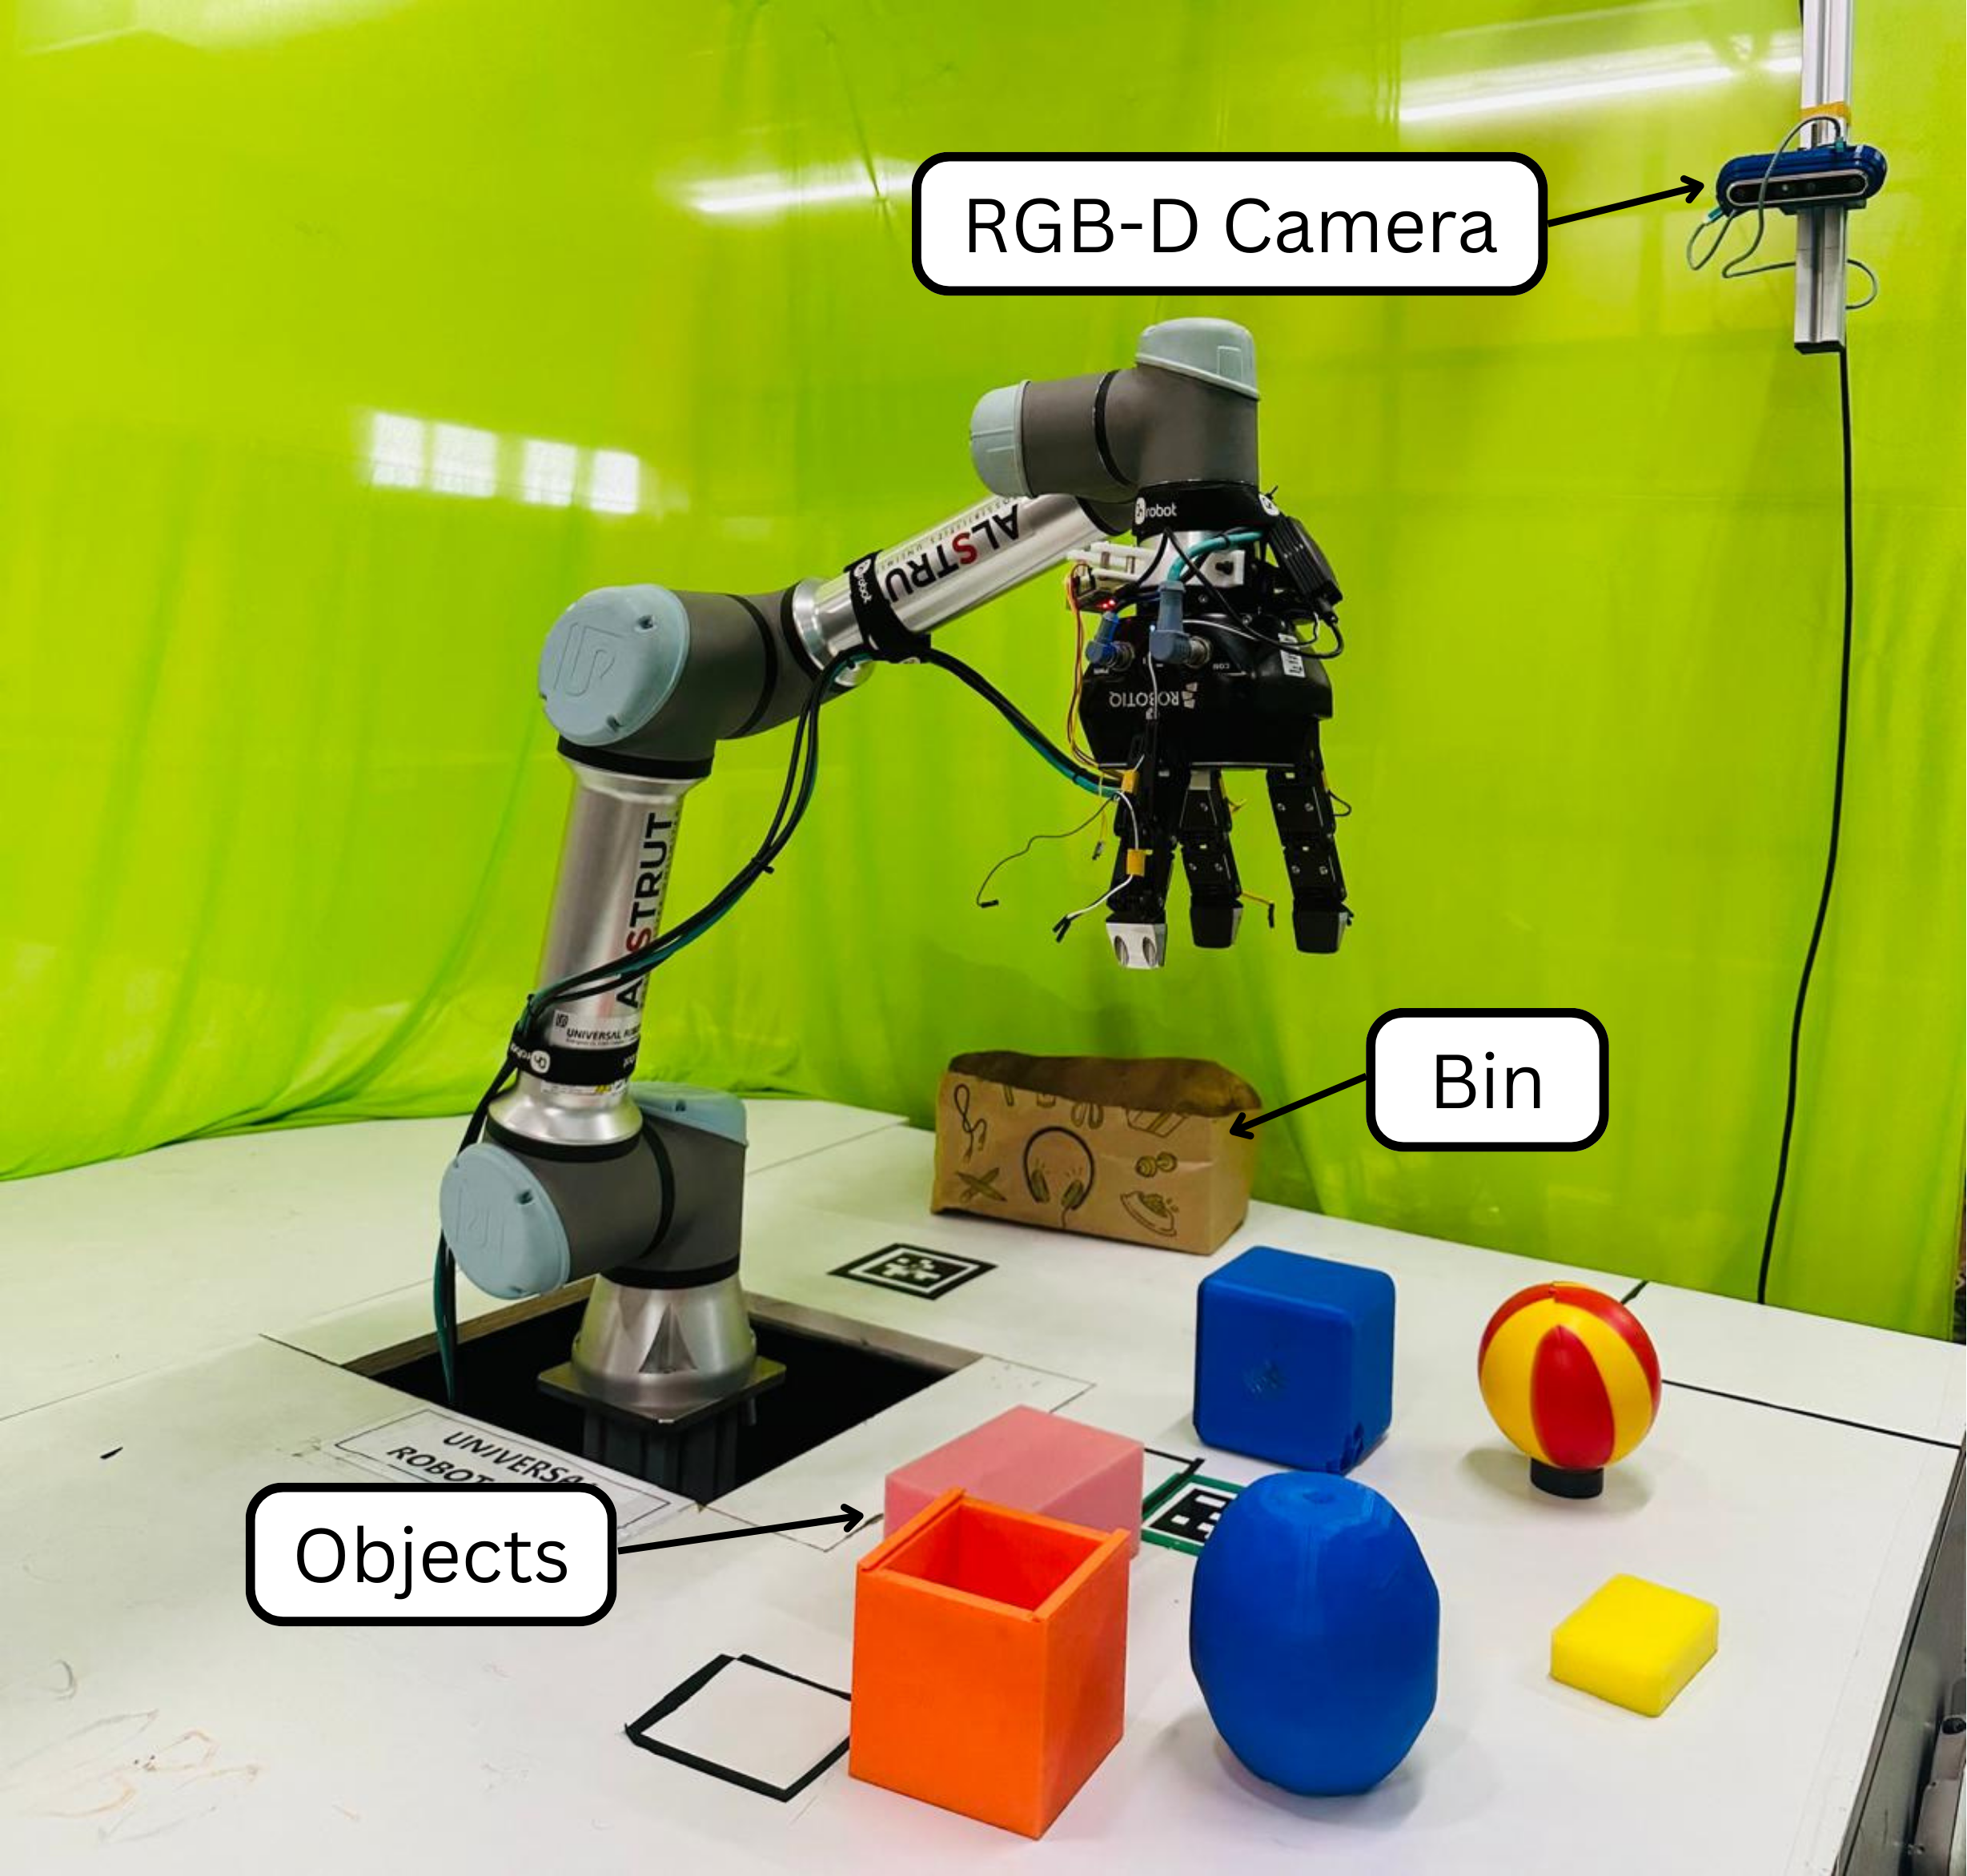
\includegraphics[width=0.5\textwidth]{real.png}
\caption{Real-world UR5 manipulation setup featuring objects of varying colours and shapes.}
\label{fig:real}
\end{figure}

Figure~\ref{fig:real} illustrates the real-world setup. An Intel RealSense D435i RGB camera is mounted to capture the gripper and workspace, and five objects of varying shapes and colours are placed in randomised configurations. Only RGB images are used for perception. Tasks are specified through natural language instructions describing the target objects and goal location.

\section{Conclusion and Future Work}

\subsection{Summary}
This report presented Recursive Belief VLA (RB-VLA), a belief-conditioned vision--language--action framework designed for long-horizon manipulation under partial observability. The central premise of the work is that long-horizon manipulation is bottlenecked not by semantic perception but by the absence of a persistent, action-conditioned representation of task progress. RB-VLA addresses this gap by introducing a fixed-size, recursively updated belief state trained with self-supervised world-model objectives, decoupling semantic grounding (delegated to a sparsely queried VLM) from causal state estimation and low-level control.

The proposed architecture combines three components: a frozen vision--language model that produces a one-shot grounded intent embedding, a recursive belief estimator that integrates observations, actions and proprioception into a 256-dimensional latent state, and a diffusion-transformer policy that generates closed-loop action chunks conditioned on both belief and intent. The belief is trained with an RSSM-style ELBO objective augmented with multi-step prediction and inverse-dynamics losses, encouraging the latent state to capture controllable, action-grounded dynamics rather than passive visual features.

\subsection{Key Findings}
Across simulation and real-world experiments, three findings stand out:

\begin{itemize}
    \item \textbf{The belief is the primary driver of long-horizon performance.} Component ablations show success rate jumping from $32.5\%$ (no belief) to $77.5\%$ (full RB-VLA) on multi-stage pick-and-place under occlusion. Belief --- not language reasoning --- governs reliable progression through stages.
    \item \textbf{Belief proximity predicts dynamical futures.} Cosine similarity in belief space correlates strongly with future action similarity ($r = 0.87$) and future visual similarity ($r = 0.78$), providing direct empirical evidence that the learned belief functions as an action-conditioned dynamical state rather than a passive memory buffer.
    \item \textbf{Episodic semantic grounding is sufficient.} Querying the VLM once per task --- rather than at every timestep --- yields more than $5\times$ lower latency than stateless baselines without sacrificing task success, validating the decoupling of intent from control.
\end{itemize}

Together with the constant-memory profile of the recursive belief, these findings demonstrate that compact, action-conditioned latent state is both necessary and largely sufficient for the long-horizon, multi-stage regime where existing observation-driven VLAs degrade most sharply.

\subsection{Future Work}
Several directions extend this work:

\paragraph{Reinforcement learning for recovery.} The current belief and policy are trained purely with self-supervised and imitation objectives. Closing the loop with online or offline reinforcement learning would let both modules co-adapt for recovery from execution failures (e.g., slips, premature releases, unintended contact) and would reduce reliance on dense teleoperation data in scenarios where high-quality demonstrations are scarce.

\paragraph{Sim-to-real with systematic domain randomisation.} While the diffusion policy adapts to real hardware via 100 trajectories of fine-tuning, broader sim-to-real transfer would benefit from systematic domain randomisation over lighting, textures, and dynamics during simulation training, together with auxiliary contact-aware self-supervision on the real robot. Combining randomisation with the action-grounded targets used to train the belief is a particularly promising direction, as it would expose the belief to a wider distribution of dynamics-relevant visual variation.

\paragraph{Bimanual and dexterous manipulation.} The belief representation is task-agnostic in form, but the current evaluation focuses on single-arm pick-and-place and stacking. Extending to bimanual coordination and multi-finger dexterous tasks would test whether the recursive belief can capture richer interaction histories such as inter-arm coordination, in-hand manipulation, and contact-rich tool use.

\paragraph{Adaptive replanning under instruction changes.} The current architecture treats the intent embedding as static across an episode. Real-world deployments often involve evolving instructions or partial replanning. Allowing the VLM to be re-invoked under explicit triggers --- task failure, instruction change, or detected belief uncertainty --- while preserving belief continuity would extend RB-VLA to interactive and human-in-the-loop settings.

\paragraph{Scaling backbones and trajectory data.} Larger VLM backbones (e.g., Qwen2.5-VL-72B) and broader trajectory corpora such as Open X-Embodiment may further improve generalisation, particularly for novel object categories and unseen instructions. The episodic VLM-querying scheme makes such scaling computationally affordable, since the cost is paid only once per task rather than at every timestep.

\paragraph{Theoretical analysis of belief sufficiency.} A formal analysis linking the learned belief to a sufficient statistic for the underlying POMDP --- and characterising the gap between the learned belief and a Bayes-optimal posterior --- remains open. Such analysis would clarify when and why belief proximity predicts future similarity, and would motivate principled regularisers in place of the present empirical loss balance.

\paragraph{Integration into pretrained VLAs.} The recursive belief module is designed as a fine-tuning layer rather than a from-scratch architecture. Integrating it into existing pretrained VLAs (e.g., $\pi_0$, OpenVLA, GR00T-N1) as a plug-in memory module is a low-cost path to upgrading deployed systems without retraining their policy stacks, and is a natural next experiment.

Taken together, these directions move RB-VLA toward a general, deployable framework for memory-aware vision--language--action control --- one in which compact, action-grounded internal state, rather than ever-growing observation context, becomes the primary substrate for long-horizon decision making.

\section*{Acknowledgments}
I would like to express my sincere gratitude to Professor Bijo Sebastian for his invaluable guidance, constant support, and encouragement throughout the course of this project.

I would also like to thank the Department of Engineering Design at the Indian Institute of Technology Madras for providing the necessary resources that made this project possible.

\bibliographystyle{IEEEtran}
\bibliography{references}

\end{document}
